% This LaTeX document needs to be compiled with XeLaTeX.
\documentclass[
  10
]{article}
\usepackage[margin=2cm,includehead=true,includefoot=true,centering,]{geometry}
\usepackage{xcolor}
\usepackage{ucharclasses}
\usepackage{hyperref}
\usepackage{amsmath,amssymb}
\usepackage{amsfonts}
\usepackage[version=4]{mhchem}
\usepackage{stmaryrd}
\usepackage{bbold}
\usepackage{polyglossia}
\usepackage{fontspec}
\usepackage{ctex}
\usepackage[export]{adjustbox}
\usepackage{tabularx}
\usepackage{booktabs}

\usepackage{setspace}
\setstretch{1.2}

\makeatletter
\@ifundefined{KOMAClassName}{% if non-KOMA class
  \IfFileExists{parskip.sty}{%
    \usepackage{parskip}
  }{% else
    \setlength{\parindent}{0pt}
    \setlength{\parskip}{6pt plus 2pt minus 1pt}}
}{% if KOMA class
  \KOMAoptions{parskip=half}}
\makeatother
\usepackage{longtable,booktabs,array}
\newcounter{none} % for unnumbered tables
\usepackage{multirow}
\usepackage{calc} % for calculating minipage widths
% Correct order of tables after \paragraph or \subparagraph
\usepackage{etoolbox}
\makeatletter
\patchcmd\longtable{\par}{\if@noskipsec\mbox{}\fi\par}{}{}
\makeatother
% Allow footnotes in longtable head/foot
\IfFileExists{footnotehyper.sty}{\usepackage{footnotehyper}}{\usepackage{footnote}}
\makesavenoteenv{longtable}
\usepackage{graphicx}
\makeatletter
\newsavebox\pandoc@box
\newcommand*\pandocbounded[1]{% scales image to fit in text height/width
  \sbox\pandoc@box{#1}%
  \Gscale@div\@tempa{\textheight}{\dimexpr\ht\pandoc@box+\dp\pandoc@box\relax}%
  \Gscale@div\@tempb{\linewidth}{\wd\pandoc@box}%
  \ifdim\@tempb\p@<\@tempa\p@\let\@tempa\@tempb\fi% select the smaller of both
  \ifdim\@tempa\p@<\p@\scalebox{\@tempa}{\usebox\pandoc@box}%
  \else\usebox{\pandoc@box}%
  \fi%
}
% Set default figure placement to htbp
\def\fps@figure{htbp}
\makeatother
\setlength{\emergencystretch}{3em} % prevent overfull lines
\providecommand{\tightlist}{%
  \setlength{\itemsep}{0pt}\setlength{\parskip}{0pt}}


\hypersetup{colorlinks=true, linkcolor=blue, filecolor=magenta, urlcolor=cyan,}
\urlstyle{same}

\usepackage{colortbl}
\definecolor{table-row-color}{HTML}{999999}
\definecolor{table-rule-color}{HTML}{999999}
%\arrayrulecolor{black!40}
\arrayrulecolor{table-rule-color}     % color of \toprule, \midrule, \bottomrule
\setlength{\aboverulesep}{0pt}
\setlength{\belowrulesep}{0pt}


\setotherlanguages{english}
\IfFontExistsTF{Source Han Serif CN}
{\newfontfamily\chinesefont{Source Han Serif CN}}
{\IfFontExistsTF{Noto Serif CJK SC}
  {\newfontfamily\chinesefont{Noto Serif CJK SC}}
  {\IfFontExistsTF{SimSun}
    {\newfontfamily\chinesefont{SimSun}}
    {\IfFontExistsTF{FangSong}
      {\newfontfamily\chinesefont{FangSong}}
      {\newfontfamily\chinesefont{Arial Unicode MS}}
}}}
\IfFontExistsTF{Times New Roman}
{\newfontfamily\englishfont{Times New Roman}}
{\IfFontExistsTF{Liberation Serif}
  {\newfontfamily\englishfont{Liberation Serif}}
  {\IfFontExistsTF{DejaVu Serif}
    {\newfontfamily\englishfont{DejaVu Serif}}
    {\newfontfamily\englishfont{Arial}}
}}


\author{}
\date{}

\begin{document}


\section{MiMo-V2.6: Scaling Reinforcement Learning Towards
Self-Improvement}\label{mimo-v2.6-scaling-reinforcement-learning-towards-self-improvement}

LLM-Core Xiaomi

\subsection{Abstract}\label{abstract}

Reinforcement learning (RL) is the central training paradigm for
advancing large foundation models towards self-improvement. This report
introduces the MiMo-V2.6 series, an omni-modal family that pushes the
frontier of model intelligence by scaling RL compute. Prior to RL, we
conduct mid-training on a broad multimodal corpus to provide ample
exploration space, and build a solid infrastructure on the pretrained
hybrid-SWA architecture to support subsequent scale-up. We scale RL
compute along three dimensions: (1) larger batches and higher
throughput, with an asynchronous training that consumes 1,568 samples
and 2.7∼3.7B tokens per step at context lengths of up to 1M; (2) more
diverse and complex environments, spanning code, general, visual, and
cyber domains under a mixture of agent harnesses; and (3) more grader
compute, via groupwise agentic grading that yields more accurate reward
signals for long-horizon tasks and steers the model towards shorter,
more token-eficient solutions. To keep training stable at scale, we
freeze the MoE router and establish a multi-layer defense against reward
hacking. We fur ther build infrastructure for mixed-task agentic RL,
including a unified trajectory representation, high-concurrency
multi-framework rollout, decoupled control and data planes, and
training-- inference consistency. We open-source the training dynamics,
RL environments, and RL frame work to facilitate reproduction and
further research on scaled RL and model self-improvement.

\pandocbounded{\includegraphics[keepaspectratio,alt={image}]{images/8142350ddbc5e79761e7dae3ce2abcc870ed6621f518abe1c2f9fb7bbbba1e8f.jpg}}

\pandocbounded{\includegraphics[keepaspectratio,alt={image}]{images/d89b08b21fc4ae915fea4d0c49c1ec0c34a66df0df2e6f6eec7165add1da8c5f.jpg}}

\pandocbounded{\includegraphics[keepaspectratio,alt={image}]{images/4214a66911c313ea87fdcb6710d81cdd603bc7b565e69fdf0470ef33dd390d82.jpg}}

\pandocbounded{\includegraphics[keepaspectratio,alt={image}]{images/f282c6e8726a01d08e55f988d178b7fec05f52cdb4501f72e84d24077e58e9c5.jpg}}

\pandocbounded{\includegraphics[keepaspectratio,alt={image}]{images/e4c74ca6f9a9384faa8383b42d62813cadf0d392f39fd2ddaef463edb24cbc3c.jpg}}

\pandocbounded{\includegraphics[keepaspectratio,alt={image}]{images/1d43d3f57ff026ba21173475e95d535090d4b4cc07e9f5111d13c5d7c8ec332f.jpg}}

Figure 1 Benchmark score per task of MiMo-V2.6-Pro and MiMo-V2.6-Flash
throughout RL training.

\subsection{Contents}\label{contents}

1 Introduction 3 2 Architecture 4 2.1 Overall Architecture . . . . . . .
. . . . . . . . . . . . . . . . . . . . . . . . . . . . . . . . . . . .
. . . . . . . . . . . . . . . . . . . . . . . . . . . . . . . . . . . .
. . . . . . 2.2 MiMo-ViT . . . . . . . . . . . . . . . . . . . . . . . .
. . . . . . . . . . . . . . . . . . . . . . . . . . . . . . . . . . . .
. . . . . . . 4 2.3 Audio Encoder 5 2.4 Speculative Decoder 5 3
Pre-Training 7 3.1 Pre-Training Setup 7 3.2 Mid-Training Setup 7 4
Scaling Reinforcement Learning 8 4.1 Scaling RL Training Computation 8
4.2 Scaling RL Environments and Harnesses 9 4.3 Groupwise Agentic
Grading 16 5 Experiments: You Only RL Once 20 5.1 Training Setup 20 5.2
Evaluation Settings 21 5.3 RL Performance 22 5.4 Router Freezing for
Stable RL 23 5.5 RL Failure Analysis 23 5.6 Broadening Capabilities via
MOPD2 24 6 RL and OPD Infrastructure 26 6.1 Agentic RL with Fine-grained
Learning Signals 26 6.2 Harness Pool and Payload Porter: Large-Batch RL
with Multiple Harnesses 27 6.3 Sample Mixer: Stable Asynchronous
Mixed-task RL 29 6.4 Training/Inference Consistency and Optimization 32
7 Open Foundations for Agentic RL 33 7.1 Distillation from MiMo-V2.6 33
7.2 RL with Open Environments 34 8 Conclusion 36 A Contributions and
Acknowledgments 44

\subsection{1 Introduction}\label{introduction}

Recursive self-improvement (RSI) envisions models that expand their
capabilities through sustained exploration and feedback. Realizing this
vision requires agents, which couple models with interactive
environments and thereby supply the multi-step trajectories and feedback
sig nals that self-improvement depends on. Towards this goal, scaling
reinforcement learning (RL) on complex agentic tasks thus opens a
concrete path. However, realizing this potential faces two major
challenges. First, RL for foundation models requires suitable model
architectures and a suficiently rich exploration space for agents.
Second, scaling RL requires sophisticated solu tions for infrastructure,
environments and grader. In this report, we introduce the MiMo-V2.6
series, including MiMo-V2.6-Pro, a 1.02T-parameter Mixture-of-Experts
model with 42B active parameters, and MiMo-V2.6-Flash, a 310B-parameter
Mixture-of-Experts model with 15B active parameters, to bridge these
gaps, taking a practical step in large-scale RL.

The architecture, pre-training, and mid-training of MiMo-V2.6 jointly
establish a powerful and eficient foundation model. Motivated by the
need to preserve global context at low computational cost, MiMo-V2.6
builds a hybrid sparse MoE Transformer backbone that interleaves Local
Sliding Window Attention (SWA) with Global Attention (GA), augmented by
a lightweight visual encoder, audio encoders. In addition, large-scale
pre-training equips the model with extensive knowledge and versatile
multimodal understanding across text, audio, and video. We further
introduce an agent-centric mid-training phase that expands the
exploration space for agentic tasks, enabling the model to discover more
efective task-solving trajectories during post-training.

Next, we scale the RL compute through a systematic, co-designed
framework spanning three key components. First, we scale batch size and
training throughput through fully asynchronous training, processing
thousands of long-horizon rollouts and billions of tokens per step at
context lengths of up to 1M. Second, we scale the diversity and
complexity of RL environments across coding, general, visual, and
cybersecurity tasks, using diverse agent harnesses and strengthening
safeguards against reward hacking. Varying both the harness and the task
improves the model generalization. Third, we introduce groupwise agentic
grading to provide more informative reward signals beyond binary test
cases. Instead of assigning the same reward to all solutions that pass
the test cases, we compare solutions within each group to distinguish
problem-solving quality and behaviors. Through our proposed Groupwise
Reward Synthesis (GRS) and Group wise Advantage Redistribution (GAR),
these fine-grained distinctions are converted into more informative
learning signals, guiding the model toward more accurate and eficient
solutions.

Realizing these at scale presents both research and engineering
challenges for infrastructure. To support flexible agentic interaction
scenarios, we design a unified trajectory representation and a penalty
mechanism that together refine the learning signal. To handle large
training batches, we sustain high-concurrency interaction across diverse
agent frameworks through a pool of harness, and decouple the control
plane from the data plane to bufer and transfer massive trajectories
carrying routing and multi-modal payloads. A sample mixing mechanism,
working together with dynamic sampling and partial rollout, stabilizes
per-task sample composition in train batches. We align the training and
inference engines on MoE routing and top-p sampling candidate sets, and
optimize both engines for RL workloads.

Scaling RL compute substantially unlocks model potential on both
verifiable tasks such as coding and less verifiable tasks such as web
development. As shown in Figure 1, both MiMo-V2.6-Pro and
MiMo-V2.6-Flash steadily improve their performance across the reported
benchmarks as training steps increase. Moreover, these gains are not
confined to a single domain, but hold consistently across diverse tasks
spanning coding on DeepSWE (Huang et al., 2026), general workflows on

AutomationBench (Shepard and Salimans, 2026), visual tasks on MiMo
Visual Coding, and cybersecurity on MiMo Cyber Bench. These gains
indicate that MiMo-V2.6 is capable of stronger complex problem solving
and more reliable performance in daily co-work scenarios, reflecting
more general agentic intelligence.

To promote research in agentic RL, we open-source a comprehensive suite
covering the key com ponents of the RL development stack, including the
lightweight model MiMo-V2.6-Distill-Qwen-9B, curated task environments
with verifiers across multiple domains, an end-to-end RL training
framework, and a composable mini-harness for flexible agentic
interactions. Together, these components provide a unified and
accessible platform for studying agentic RL under diverse tasks,
environments, and agent configurations, while reducing the engineering
barriers to reproducing and extending large-scale RL experiments.
Experiments with MiMo-V2.6-Distill-Qwen-9B demonstrate consistent RL
gains across diverse tasks and agent harnesses, validating the
efectiveness and generality of the proposed suite. We hope this
open-source suite can serve as a fair, strong, and reproducible baseline
for the community, enabling systematic investigation of agentic RL and
advancing research toward recursive self-improvement.

\subsection{2 Architecture}\label{architecture}

\subsection{2.1 Overall Architecture}\label{overall-architecture}

As illustrated in Figure 2, MiMo-V2.6 follows a standard Transformer
(Vaswani et al., 2017) backbone, augmented with visual and audio
encoders connected through lightweight projectors.

The text backbone of MiMo-V2.6 is mainly composed of repeated hybrid
blocks that interleave Local Sliding Window Attention (SWA) and Global
Attention (GA). It stacks � hybrid blocks, each structured with �
consecutive SWA blocks followed by a GA block. The only exception is the
very first Transformer block, which uses global attention with a dense
Feed-Forward Network (FFN) to stabilize early representation learning.
The sliding window size � used in MiMo-V2.6 is 128. Both the SWA block
and the GA block utilize a sparse MoE FFN without shared experts.
MiMo-V2.6 also integrates an SWA and dense FFN based MTP (Gloeckle et
al., 2024; Liu et al., 2024; Xia et al., 2025) to improve model
performance during pre-training. A more comprehensive description of the
text backbone architecture can be found in Core Team et al.~(2026). The
model configurations are shown in Table 1.

\subsection{2.2 MiMo-ViT}\label{mimo-vit}

MiMo-ViT adopts a hybrid attention architecture. It replaces fixed,
non-overlapping window attention in MiMo-VL-7B (Yue et al., 2025) with
sink-augmented SWA, enabling information exchange across window
boundaries over successive layers and mitigating visual fragmentation.
Local SWA layers alternate between row-major and column-major token
serialization to support information propagation along both spatial
axes. Finally, GA layers are inserted periodically to aggregate global
context directly. This design substantially reduces the computational
cost of high-resolution visual processing while achieving performance
comparable to GA ViTs. Please refer to He et al.~(2026) for more
analysis. To pre-train MiMo-ViT from scratch, we pair it with a small
pre-trained LLM and optimize the resulting VLM solely on multimodal
understanding data using a cross-entropy objective. This simple recipe
avoids auxiliary objectives such as contrastive learning, making
pre-training eficient and scalable. Crucially, the LLM remains trainable
to provide stable, semantically meaningful gradients to the ViT. After
pre-training on more than 4T image tokens, MiMo-ViT learns strong visual
representations and serves as a robust foundation for MiMo-V2.6.

\pandocbounded{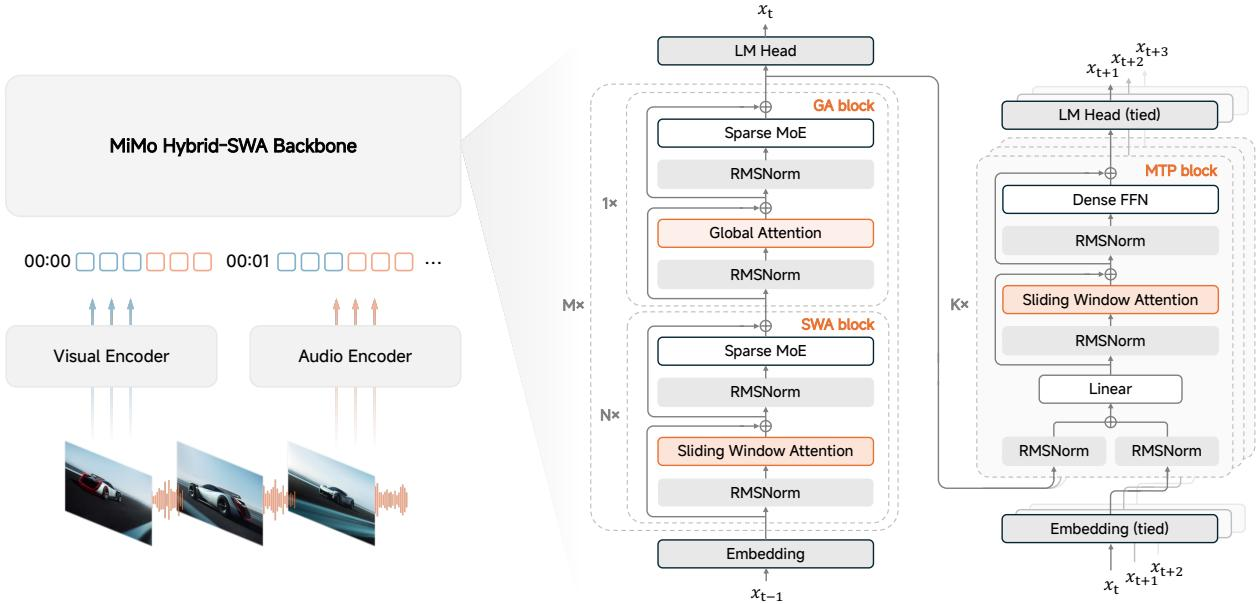
\includegraphics[keepaspectratio,alt={image}]{images/80846bdb6b58805054d6906fc420abb05a89328851d452ae336116b75a19724e.jpg}}

Figure 2 Overall architecture of MiMo-V2.6. Audio, visual, and text
inputs are mapped into a shared token sequence and processed by the MiMo
Hybrid-SWA backbone, followed by the language-modeling head and
multi-token prediction (MTP) blocks.

\subsection{2.3 Audio Encoder}\label{audio-encoder}

Audio encoding in MiMo-V2.6 consists of two stages: audio tokenization
with the Audio Tokenizer, followed by patch encoding. The Audio
Tokenizer encoder first processes log-mel spectrograms through a
two-layer convolutional frontend that halves the frame rate. The
resulting sequence is then passed through a Transformer with a causal
hybrid attention architecture that interleaves SWA and GA layers. SWA
layers capture local temporal dependencies, while GA layers aggregate
context across the full preceding sequence. A subsequent downsampling
convolution further halves the frame rate to 25 Hz, after which a
20-layer residual vector quantizer (RVQ) represents each frame as 20
discrete audio tokens. The Audio Tokenizer follows the training recipe
of MiMo-Audio (Xiaomi, 2025) and is trained on 20 million hours of audio
spanning speech, music, and other audio content.

The audio patch encoder follows the architectural design of MiMo-Audio
and is trained jointly with the text backbone. At each time step, the
audio tokens are embedded using separate embedding tables, one per RVQ
codebook, and the resulting embeddings are summed to form a single frame
representation. Every four consecutive frames are grouped into an audio
patch and processed by a Transformer with bidirectional self-attention
confined to that patch. The four out put representations are then
concatenated and linearly projected into a single backbone input
embedding, reducing the audio sequence rate from 25 Hz to 6.25 Hz.

\subsection{2.4 Speculative Decoder}\label{speculative-decoder}

Speculative decoding in MiMo-V2.6 uses a multi-token prediction (MTP)
module following the block difusion design of DFlash (Chen et al.,
2026). The drafter comprises 5 Transformer layers with dense
feed-forward networks. Conditioned on backbone hidden features and a
clean anchor token, it predicts 7 subsequent tokens in a single forward
pass for parallel verification by the backbone. All draft layers use
sliding-window attention (SWA) with grouped queries to limit attention
computation and KV-cache size. Tokens attend bidirectionally within
their draft block and to at most 1,024 backbone context positions
preceding the anchor.

{\def\LTcaptype{none} % do not increment counter
\begin{longtable}[]{@{}llll@{}}
\toprule\noalign{}
\endhead
\bottomrule\noalign{}
\endlastfoot
Block & Configuration & MiMo-V2.6-Flash & MiMo-V2.6-Pro \\
\multirow{9}{*}{Main Block} & Layers (Total/SWA/GA) & 48/39/9 &
70/60/10 \\
& Hidden Size & 4096 & 6144 \\
& SWA Heads (Q/KV) & 64/8 & 128/8 \\
& Sliding Window Size & 128 & 128 \\
& GA Heads (Q/KV) & 64/4 & 128/8 \\
& Head Dimensions (QK/V) & 192/128 & 192/128 \\
& Experts (Total/Activated) & 256/8 & 384/8 \\
& \# Total Parameters & 310B & 1.02T \\
& \# Active Parameters & 15B & 42B \\
\multirow{8}{*}{MiMo-ViT} & Layers (Total/SWA/GA) &
\multicolumn{2}{l@{}}{%
28/24/4} \\
& Hidden Size & \multicolumn{2}{l@{}}{%
1280} \\
& Attention Heads (Q/KV) & \multicolumn{2}{l@{}}{%
32/8} \\
& Head Dimension & \multicolumn{2}{l@{}}{%
64} \\
& Patch Size (T \textbackslash times H \textbackslash times W) &
\multicolumn{2}{l@{}}{%
2 \textbackslash times 16 \textbackslash times 16} \\
& Sliding Window Size (Left/Right) & \multicolumn{2}{l@{}}{%
64/64} \\
& Spatial Merge Size & \multicolumn{2}{l@{}}{%
2 \textbackslash times 2} \\
& \# Parameters & \multicolumn{2}{l@{}}{%
681M} \\
\multirow{8}{*}{Audio Tokenizer Encoder} & Layers (Total/SWA/GA) &
\multicolumn{2}{l@{}}{%
24/12/12} \\
& Hidden Size & \multicolumn{2}{l@{}}{%
1024} \\
& Attention Heads (Q/KV) & \multicolumn{2}{l@{}}{%
16/16} \\
& Head Dimension & \multicolumn{2}{l@{}}{%
64} \\
& Mel Bins & \multicolumn{2}{l@{}}{%
128} \\
& Sliding Window Size & \multicolumn{2}{l@{}}{%
128} \\
& Codebooks & \multicolumn{2}{l@{}}{%
20} \\
& \# Parameters & \multicolumn{2}{l@{}}{%
308M} \\
\multirow{6}{*}{Audio Patch Encoder} & Layers & \multicolumn{2}{l@{}}{%
6} \\
& Hidden Size & \multicolumn{2}{l@{}}{%
1024} \\
& Attention Heads (Q/KV) & \multicolumn{2}{l@{}}{%
16/16} \\
& Head Dimension & \multicolumn{2}{l@{}}{%
64} \\
& Attention Group Size & \multicolumn{2}{l@{}}{%
4} \\
& \# Parameters & \multicolumn{2}{l@{}}{%
127M} \\
\multirow{6}{*}{Speculative Decoder} & Layers (Total/SWA/GA) & 5/5/0 &
5/5/0 \\
& Hidden Size & 4096 & 6144 \\
& SWA Heads (Q/KV) & 64/8 & 128/8 \\
& Sliding Window Size & 1024 & 1024 \\
& GA Heads (Q/KV) & 64/4 & 128/8 \\
& Head Dimensions (QK/V) & 128/128 & 128/128 \\
\end{longtable}
}

Table 1 Detailed model configurations of MiMo-V2.6-Flash and
MiMo-V2.6-Pro. Main block layer counts exclude MTP modules. Encoder
parameter counts include input embeddings but exclude projectors. The
audio tokenizer encoder parameter count excludes EMA codebooks.

\subsection{3 Pre-Training}\label{pre-training}

\subsection{3.1 Pre-Training Setup}\label{pre-training-setup}

The pre-training corpus of MiMo-V2.6 spans text, vision, and audio. The
text corpus draws from a broad range of sources, including public web
content, books, academic papers, code, and STEM materials. The vision
corpus includes image-captioning, grounding, OCR, GUI, conversation,
video, and visual-coding data. For audio, we curate diverse,
high-quality data at scale and organize the data into three task
formats: speech-text interleaving, automatic speech recognition (ASR),
and general audio captioning.

We adopt a two-stage pre-training strategy. In the first stage, we train
the language backbone on text-only data to establish strong foundational
language capabilities. In the second stage, we integrate the backbone
with our in-house pre-trained ViT and audio encoder and jointly train
the full model on omni-modal data, enabling it to understand images,
videos, and audio.

We begin pre-training with a context length of 32K tokens and extend it
to 256K partway through training. MiMo-V2.6-Flash is trained on 48T
tokens, comprising 26T tokens in the text stage and 22T in the omni
stage. MiMo-V2.6-Pro is trained on 30T tokens, with 27T and 3T tokens in
the two stages, respectively. We employ the AdamW optimizer in the
pre-training of MiMo-V2.6.

\subsection{3.2 Mid-Training Setup}\label{mid-training-setup}

Pre-training builds broad knowledge and general understanding across
text, vision, and audio. Mid-training bridges this general foundation
and subsequent large-scale RL by further developing the model's agentic
abilities, extending long-context support, and adapting the optimization
setup for large-batch training.

To this end, we train the MiMo-V2.6 model series on a diverse,
agent-centric data mixture. Its diversity spans both task domains and
data modalities, combining realistic agent trajectories across coding,
general, visual, and research tasks with high-quality text,
repository-level code, and image, video, and audio data. Training
proceeds in two stages: we first train with a 256K context length,
allocating the majority of compute to this stage, and then extend the
context length to 1M in the final stage.

Our base model was pre-trained with AdamW, but our preliminary
experiments showed diminishing optimization eficiency as the batch size
increased in mixed-task RL. Unlike AdamW, which adapts parameters
element-wise, Muon leverages the matrix structure of hidden weights by
orthogonalizing their updates (Jordan et al., 2024). This matrix-based
update retains stronger data eficiency beyond the critical-batch-size
regime, making Muon particularly attractive for largebatch training (Liu
et al., 2025b; Shah et al., 2025). We therefore switch to a variant of
Muon optimizer, Muown, for the hidden weight matrices during
mid-training to prepare the model for subsequent large-batch RL. Muown
augments Muon with explicit row-norm control, mitigating spectral-norm
drift and reducing sensitivity to weight decay at negligible overhead
(Lion et al., 2026). Embeddings, the LM head, and the MoE router
continue to use AdamW.

Prior work reports that switching an Adam-pre-trained model to Muon
training can cause optimizer mismatch and degraded performance (Qu et
al., 2026). Nevertheless, during our midtraining, we observe no loss
spike throughout the training process.

We employ MXFP4 quantization-aware training (QAT) during mid-training,
allowing the model to adapt to low-precision computation while
preserving model quality.

\pandocbounded{\includegraphics[keepaspectratio,alt={image}]{images/7645994004a4eda93e41f6199313a6d8e20dcac99f9c1bf26c87bf592bed315d.jpg}}

\pandocbounded{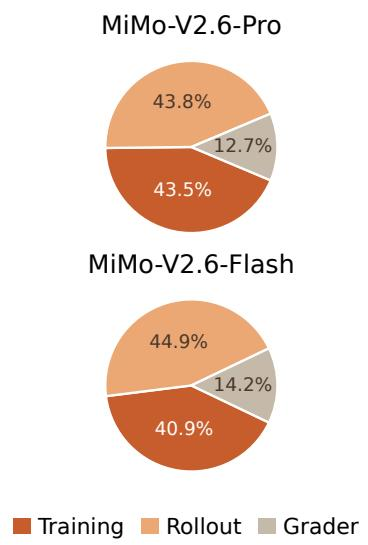
\includegraphics[keepaspectratio,alt={image}]{images/c536e6e9f740d8147a897d751ac2d1b6346bce68fe0c475d79b14eafc932c115.jpg}}

Figure 3 Left: average@3 score on DeepSWE v1.1 versus cumulative RL
cost. Right: training, rollout, and grader cost shares for MiMo-V2.6-Pro
and MiMo-V2.6-Flash.

\subsection{4 Scaling Reinforcement
Learning}\label{scaling-reinforcement-learning}

In this release, we continue to push the boundaries of post-training
algorithms, with a particular focus on scaling RL compute. Following a
short supervised fine-tuning (SFT) stage, we scale RL along three
dimensions, training computation (§4.1), environments and agent
harnesses (§4.2), and grader computation (§4.3), achieving a fundamental
leap in model capabilities.

\subsection{4.1 Scaling RL Training
Computation}\label{scaling-rl-training-computation}

We scale RL computation across thousands of GPUs in a single run,
spending \$2.6M and \$0.9M on RL post-training for MiMo-V2.6-Pro and
MiMo-V2.6-Flash, respectively. We use a large training batch: 1,568
prompts with group size �=16, so each step rolls out 25K sequences that
amount to 2.7B--3.7B training tokens (roughly 110K--150K tokens per
sequence). The left panel of Figure 3 shows the benefit of scaling RL
computation. The average@3 score on the DeepSWE benchmark (Huang and
Jiang, 2026) rises steadily with cumulative cost for both models: over
the course of \(\mathrm { R L } ,\) MiMo-V2.6-Pro improves from 58.4 to
72.6 and MiMo-V2.6-Flash from 48.7 to 65.7. The computation splits into
three parts: rollout, grading, and training. Such scaling calls for
solid infrastructure to keep training eficient and stable.

We form the RL learning objective as follows:

\[
\mathcal {L} (\theta) = - \mathbb {E} _ {q \sim \bigcup_ {d} \mathcal {D} _ {d}, \{o _ {i} \} _ {i = 1} ^ {G} \sim \mu_ {\theta_ {\mathrm{old}}} (\cdot | q)} \left[ \frac {1}{\sum_ {i = 1} ^ {G} | o _ {i} |} \sum_ {i = 1} ^ {G} \sum_ {t = 1} ^ {| o _ {i} |} r _ {i, t} M _ {i, t} A _ {i} \log \pi_ {\theta} (o _ {i, t} | q, o _ {i, <   t}) \right],\tag{1}
\]

where � denotes the importance sampling ratio, � is the token-level
mask, and � is the advantage. The computation can be decomposed into
three parts. The first is rollout: for every prompt drawn from the union
of task datasets \(\cup _ { d } \mathcal { D } _ { d }\) , the rollout
policy \(\mu _ { \theta _ { \mathrm { o l d } } }\) generates a group of
� candidate solutions \{� \}. The second is grading: we invest
additional compute in agentic evaluation to distinguish efective
solutions and behaviors from flawed ones, beyond what binary test
outcomes reveal. These judgments inform the advantages \(A _ { i } ,\)
enabling more accurate credit assignment across trajectories. The third
is training: the collected tokens update � through the gradient of log
\(\pi _ { \theta } ( o _ { i , t } ~ \mid ~ q , o _ { i , < t } )\) ,
with prompt-mean aggregation. The right panel of Figure 3 breaks down
the cost of MiMo-V2.6-Pro by where the compute goes: rollout consumes
43.8\% and training 43.5\%, while the grader takes the remaining 12.7\%.
A large batch draws from diverse RL tasks spanning various environments
and harnesses within one run (Section 4.2). We also scale the grader to
provide fine-grained learning signals (Section 4.3).

A large batch is good for scaling out GPUs: rollout parallelizes over
sequences and training shards the batch across data-parallel ranks, so
throughput grows with the GPU count. With HBM mostly occupied by the
running batch, we can keep a high arithmetic intensity to fully use the
GPU in roll out. Since rollout and grading have a long tail, we use
partial rollout (Kimi Team, 2025) to keep the running batch saturated:
when we collect a training batch, we leave the in-flight sequences
interrupted and resume them in the next rollout phase. The cost is
re-prefill: a continuation must rebuild its KV cache after each policy
update, so batch size and partial rollout are chosen together---a large
batch amortizes the re-prefill. To support stable RL training,
train--inference consistency is ensured by R3 (Ma et al., 2025) and the
replay of top-p sampling candidate sets (Liu et al., 2025a; The
Microsoft AI Team, 2026). To ensure that all samples contribute to
training with efective gradients, we incorporate a dynamic sampler (Yu
et al., 2025) to filter groups that are all-pass or all-fail. In
multi-task RL, we implement a Sample Mixer to ensure eficient and stable
training batch distribution given various rollout durations and pass
rates of diferent tasks. To pack the trajectories from rollout into
large training batches (2.7B--3.7B tokens), we decou ple the data plane
and control plane. The infrastructure behind these designs is described
in Section 6.

\subsection{4.2 Scaling RL Environments and
Harnesses}\label{scaling-rl-environments-and-harnesses}

Scaling agentic RL requires diverse environments that reflect real-world
tasks, support reproducible execution at training scale, and provide
rewards aligned with task objectives. Meeting these requirements jointly
is challenging: realistic workflows involve heterogeneous tools and
complex state, while automated graders may be incomplete, inconsistent,
or vulnerable to exploitation. We therefore invest in large-scale
environment synthesis and curation across coding (§4.2.1), general
professional workflows (§4.2.2), visual artifacts (§4.2.3), and
cybersecurity (§4.2.4), emphasizing supervision quality. This subsection
describes how we construct tasks and environments across these domains,
the harnesses through which agents interact with them (§4.2.5), and the
execution checks, rollout-based audits, and adversarial testing used to
improve reward reliability and mitigate reward hacking before and during
training (§4.2.6).

\subsection{4.2.1 Code Agent Tasks}\label{code-agent-tasks}

Coding tasks are particularly well suited to RL, as candidate solutions
can be executed and evaluated through automated tests, providing
feedback at scale. However, executable evaluation alone does not
guarantee reliable supervision: tests may overlook required behavior,
reject valid implementations, or yield inconsistent outcomes across
executions. The central challenge is therefore to scale task
construction while ensuring that rewards faithfully reflect task
correctness. Moti vated by this, we devote substantial efort to building
a scalable synthesis and curation pipeline for coding-agent tasks, with
an emphasis on the accuracy and robustness of supervision. Figure 4
summarizes the task synthesis pathways and the checks used to assess
supervision accuracy and robustness.

Scalable Task Synthesis from Diverse Sources We scale task construction
through five complementary synthesis pathways, designed to cover
heterogeneous programming languages, development settings, and task
horizons. First, in GitHub-based synthesis, we collect pull requests and
their associated issues and apply heuristic and model-assisted filters
to remove duplicate, malformed, or non-reproducible candidates. When a
pull request is linked to an issue that provides a suficiently complete
description of the intended change, we use the issue as the task
specification. Other wise, an LLM reconstructs an issue-style
specification from the reference patch and the surrounding repository
context, while being explicitly instructed to omit
implementation-specific details that could reveal the solution. Second,
to capture everyday development workflows, including interactive ``vibe
coding'' scenarios, we collect real-world development requests
contributed by employees within our organization. These requests cover
common activities such as feature implementation, refactoring,
debugging, and repository maintenance, for which agents generate and
implement test cases that operationalize the requested behavior. Third,
specification-driven tasks emphasize code generation under detailed,
multi-constraint requirements, allowing us to evaluate whether models
can faithfully translate complex specifications into executable
implementations. Fourth, in source-code-driven synthesis, we use
CodeMidas (Ye et al., 2026) to derive tasks from functionality
implemented in existing codebases. Agents identify candidate
functionality and translate its observable behavior into task
specifications and executable environments, this pathway enables
scalable task construction across diverse repositories without requiring
issues, pull requests, or other development artifacts. For long-horizon
software-engineering tasks, agents iteratively elaborate task
requirements, expand the scope of the required changes, introduce
dependencies across components, and construct tests that exercise the
resulting multi-step behavior. We also include and filter samples from
public sources (Badertdinov et al., 2026; PrimeIntellect, 2026; Tao et
al., 2026; Yang et al., 2026b; Zan et al., 2025; Zhao et al., 2026) and
licensed data vendors to further enrich the task distribution.
Collectively, these pathways produce tasks spanning a broad range of
programming languages, development contexts, imple mentation
complexities, and task horizons.

\pandocbounded{\includegraphics[keepaspectratio,alt={image}]{images/b22f5313a229f8e52b12250ce921a62b490d786c88e0df36a6e98f5971b6dd66.jpg}}

Figure 4 The overall code agent task scaling pipeline. We build tasks
from diverse sources and go through rigorous assessment stages to ensure
the supervision is accurate and robust.

Accuracy of Supervision We align the behavioral scope of each task
specification with that of its unit tests. The goal is to accept
implementations that satisfy the specification and reject those that
violate it, without requiring incidental details of the reference
implementation. We review tasks for insuficient coverage and overly
restrictive checks. In particular, tests that enforce re quirements
absent from the specification are revised or removed. As inspection
alone may miss discrepancies between specifications and tests, we
further assess their alignment through rollout based auditing. Each task
is attempted four times by a coding agent. An auditing agent receives
all four rollouts in a shared workspace containing the problem
statement, tests, reference patch, and each rollout's submitted patch,
test output, and full conversation log. The auditor first articulates
what a correct solution requires and assesses whether the tests capture
those requirements. It then evaluates each submitted solution against
the specification using its patch and conversation log, and compares
this assessment with the observed reward. A passing solution judged
incorrect is flagged as a potential false positive, suggesting
incomplete verification. A failing solution judged correct is flagged as
a potential false negative, suggesting overly restrictive tests or
execution failures. These disagreements identify tasks requiring further
review and provide concrete evidence of possible mismatches between the
intended behavior and the implemented verification.

Robustness of Supervision We check reward stability through repeated
execution. For those tasks with reference patch, we ensure fail-to-pass
(F2P) tests must fail and pass-to-pass (P2P) tests must pass before
applying the reference patch; after the patch, both must pass. We
require these outcomes to remain stable across eight reruns, screening
for flaky tests and environmentinduced reward fluctuations. We also
reuse the previous rollout pipeline to collect agent trajectories to
investigate potential reward hacking. The submitted patches and
conversation logs provide evidence of how agents obtained their rewards,
helping identify unintended shortcuts or exploitation of the environment
and evaluation process. These checks complement the as sessment of
solution correctness and inform the broader reward-hacking mitigation
procedures described below.

Together, these procedures support the construction of a diverse
coding-task corpus under a consistent standard of supervision quality.
Specification--test alignment targets the fidelity of the reward signal,
repeated execution checks its stability, and rollout-based auditing
probes whether it agrees with an independent assessment of solution
correctness. Our objective is to make this combination scalable, so that
RL training can benefit from broad task coverage while encouraging
agents to satisfy the intended requirements rather than exploit gaps in
evaluation.

\subsection{4.2.2 General Agent Tasks}\label{general-agent-tasks}

We extend agent capabilities to real-world professional workflows across
diverse domains, whose workflows require agents to analyze heterogeneous
documents, use specialized software, and produce deliverables that meet
domain-specific standards. We synthesize environments that support such
workflows, then construct challenging tasks with verifiable outcomes.
Figure 5 summarizes this pipeline, including environment construction,
task synthesis, and iterative rubric refinement.

Environment Design A general-agent environment typically consists of a
workspace and a set of software tools, accessible through interfaces
such as MCP, APIs, CLIs, and GUIs. Our design balances realism with the
requirements of large-scale RL: files, software behavior, and underlying
data should reflect professional practice, while execution must remain
local and environments must be easy to reset. We therefore collect
real-world files for direct inclusion or as references for synthesis,
and use an automated multi-agent workflow to build local software mocks
that reproduce supported operations, state changes, output formats, and
error responses. Tools that already operate without external services
are integrated directly. All state is stored locally, and each rollout
runs in an isolated sandbox that can be restored to a fixed initial
state. This avoids network variability and service limits while
supporting reproducible execution.

\pandocbounded{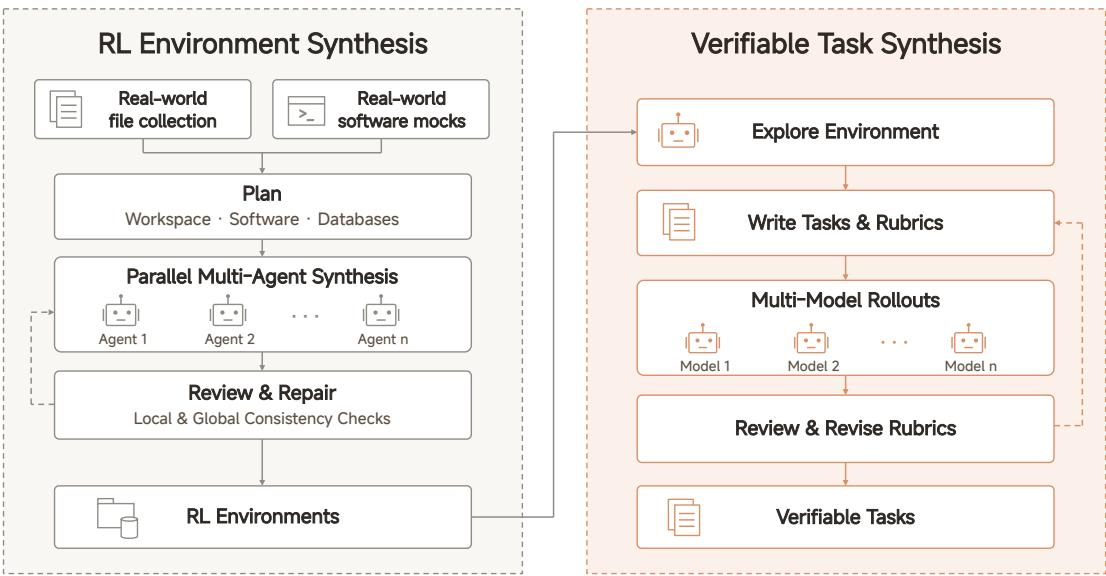
\includegraphics[keepaspectratio,alt={image}]{images/b76f04bc649fcf09d095412b001d307056b1a741e68b97a0e7aef62f9b590239.jpg}}

Figure 5 The overall general-agent environment and verifiable-task
synthesis pipeline. We first construct realistic, resettable
environments from real-world files and software mocks. Agents then
explore these environments and synthesize tasks with verifiable rubrics.

Environment Synthesis To assemble these components into coherent
scenarios, a planning agent specifies the workspace structure, selects
appropriate tools, and plans file and database contents. Web search
grounds the plan in real-world information, while relationships across
files and between files and database records support subsequent
multi-hop reasoning and cross-validation. Multiple agents then generate
files and populate databases in parallel, following the shared plan and
each mock's data specification. A review agent checks individual
artifacts and global consistency, including entity names, numerical
reconciliation, timelines, and references. Iterative repair resolves
inconsistencies before task construction. The workspace and tool
configuration vary by scenario, so each environment reflects the
relevant working practices without requiring every available file type
or software interface.

Task Synthesis and Verification We survey common professional tasks and
combine and generalize them into seed tasks. An agent explores each
environment and uses these seeds to construct tasks suited to its
contents and tools. Task completion is evaluated using atomic, binary
rubric items: code-based checks verify deterministic properties, such as
database values and deliverable formats, while LLM-based checks assess
more open-ended content. For LLM-based items, agreement across repeated
judgments by the same model and across diferent judge models helps
identify ambiguity.

Consistency alone does not establish that rubrics capture task
completion. We therefore collect rollouts from models with diferent
capability levels and have a review agent examine their trajectories,
execution results, and rubric judgments. The reviewer revises overly
restrictive criteria that reject valid solutions and overly permissive
criteria that accept incomplete ones. To test resistance to reward
hacking, we include negative checks for unintended changes to unrelated
files or databases and construct adversarial solutions that appear
correct without actually solving the task. During RL, a self-hosted
MiMo-V2.6-SFT model serves as the grader to support stable scoring. This
process yields thousands of environments and diverse, verifiable tasks,
which we combine with other tasks for RL training.

\subsection{4.2.3 Visual Agent Tasks}\label{visual-agent-tasks}

To empower agents to shape the digital world through creative expression
and precise visual control, we curate a diverse suite of visual tasks in
which agents work with a broad range of artifacts, such as websites,
interactive applications, games, 3D scenes, slides, SVG, videos and
Figma designs. We organize these tasks into two complementary
categories: open-ended design and high-fidelity visual replication.
Together, they develop the model's ability to produce reliable
implementations with strong aesthetic quality and precise visual
control.

Open-ended design seeks to produce aesthetically compelling visual
artifacts that satisfy user intent. The diversity ofvalid creative
solutions makes aesthetic quality dificult to capture through fixed
rules alone. We therefore combine pointwise and groupwise grading to
establish consistent quality standards while rewarding relative
improvements in aesthetic quality. Specifically, we first iteratively
refine pointwise rubrics for runtime correctness, instruction adherence,
layout integrity, and basic aesthetic quality. Once these rubrics
stabilize, we introduce groupwise grading that jointly compares the
rendered artifacts within each rollout group for the same query,
identifying clearly stronger and weaker candidates and assigning rewards
accordingly.

High-fidelity visual replication aims to faithfully reproduce a
specified visual target. Compared to open-ended design, the explicit
reference enables more direct evaluation of visual fidelity. We grade
these tasks primarily through rule-based similarity metrics, such as
pixel-level similarity between rendered artifacts and their references,
supplemented by LLM-based judging for holistic visual assessment.
Together, these signals support efective scaling of reinforcement
learning on visual replication tasks.

\subsection{4.2.4 Cybersecurity Agent
Tasks}\label{cybersecurity-agent-tasks}

We train cyber agents with RL on real-world vulnerability reproduction:
given a project and a target bug, the agent must construct an input that
triggers it. This foundational ofensivesecurity skill underlies exploit
development, privilege escalation, and CTF challenges. It is also well
suited to RL at scale: OSS-Fuzz supplies tens of thousands of manually
confirmed instances, a volume unmatched by other security tasks. The
dificulty is not triggering a crash, since complex C/C++ projects expose
dozens of reachable crash paths, but triggering the specific
vulnerability described. Verification must therefore separate the
intended bug from unrelated crashes, and because it doubles as the RL
reward, it must be accurate, deterministic, and cheap.

Existing oracles fall short. Fix-binary diferential testing, as used in
CyberGym (Wang et al., 2025), accepts a PoC that crashes the vulnerable
binary but not the patched one; an incomplete patch rejects correct
PoCs, and unrelated changes between the two commits flip verdicts for
rea sons unconnected to the bug. Either error corrupts the training
gradient. LLM-based judging returns diferent verdicts for the same PoC
across runs and cannot serve as a stable reward. We instead extract two
attributes from the ground-truth sanitizer (ASan/MSan/UBSan) report: the
vulnerability type (e.g., heap-bufer-overflow) and the crash location
(the topmost project-level stack frame). A PoC is accepted if its crash
matches both under rule-based string matching, which is deterministic,
reproducible, and computationally trivial. The task description is
derived from the same report, stating the exact type and function in
which the crash must occur, so description and verification share a
single source of truth; CyberGym's LLM-generated descriptions, by
contrast, are often too broad (e.g., ``bufer overflow in libxml2'') or
simply wrong.

For each vulnerability we check out the source at the reported commit,
build the fuzzing harness, and give the agent the complete runtime
environment: full source plus the compiled harness binary. CyberGym
withholds the binary, restricting agents to source-only analysis;
providing it mirrors real vulnerability analysis, where a researcher
runs the target under a debugger, inspects memory, and crafts mutations
from runtime observations.

\subsection{4.2.5 Multi-Harness Training}\label{multi-harness-training}

Agent harnesses difer in module design and are selected or built to meet
diferent application needs. Models must therefore adapt to diverse
interaction mechanisms, including those of harnesses unseen during
training, making cross-harness generalization an important capability.

Training exclusively within a single harness may couple task-solving
strategies to harness-specific implementations and limiting transfer. We
therefore treat harness diversity as an additional training dimension
alongside diversity in tasks and environments. A natural approach is to
train on several production harnesses such as MiMo Code and Codex.
However, this is a poor fit for RL in practice. First, production
harnesses wrap the agent loop with engineering safeguards and multi-step
workflows, and steer the model with numerous constraint and instruction
prompts. These extras fall outside the task-completion reward signal,
making credit assignment unreliable and leaving reward-unmeasured
requirements to simply be ignored. Second, their modules are tightly
coupled rather than independently configurable, so one cannot vary a
single interaction mechanism in isolation or assemble diversity by
controlled recombination.

To this end, we propose multi-harness training with carefully designed
mini-harnesses. All miniharnesses start from the same minimal agent
loop, which already includes the components needed for task
completion---system prompt, tools, and context management. These modules
stay minimal and decoupled, so implementations can be freely recombined
and harness expansion remains controllable, safe, and clean. We then
derive diverse, task-adapted mini-harness configurations for Code,
General, Visual, and Cyber. The resulting training distribution is
diverse yet controllable, supporting analysis of individual harness
mechanisms and encouraging transferable task-solving strategies.

\subsection{4.2.6 Reward Hacking
Mitigation}\label{reward-hacking-mitigation}

RL relies on rewards to measure task success, but agents can sometimes
earn high rewards by exploiting the environment or the evaluation
process. This behavior, known as reward hacking, can be reinforced
during training, increasing scores without improving task performance.
For common coding agent tasks like repository-repair, a recurring
failure mode is solution leakage: agents obtain a published fix beyond
the intended task context and use it to construct a patch. Table 2 links
each task request to the agent's stated intent and subsequent action
across five repositories. Such behavior can satisfy the test-based
reward without demonstrating that the agent derived the repair from the
bug report and the assigned checkout. Followingly, we introduce our
mitigation combining mid-training alignment data with RL environment
preparation, adversarial screening, and auditing throughout training.

Mid-Training Alignment Data In early experiments, we observed a tendency
toward reward hacking in MiMo. To mitigate this behavior, we synthesized
a set of training examples from these cases and included them in
mid-training. For each case, MiMo reflects on the faulty reasoning,
revises the relevant turn, and continues with actions grounded in the
task specification. The revised reasoning keeps the original error
recognizable and makes the correction explicit. We found that adding
these examples improved the model's alignment.

Environment Preparation In coding tasks, agents may pass tests by
recovering leaked solutions from the environment or retrieving existing
solutions over the network. Building a project with the reference patch
applied during environment construction can leave behind artifacts that
reveal the solution. We therefore remove build logs, verifier outputs,
residual patches, and projectgenerated binaries or bytecode that could
expose it. We also clean caches that may contain solution information,
including those outside the repository, while preserving third-party
dependencies needed for ofline rebuilding. For every task, we retain Git
history up to and including the base commit, removing later commits and
their associated references. We enforce containerlevel network isolation
to restrict access to upstream fixes and alternative package versions
that may contain the solution. These safeguards are accompanied by
explicit instructions against retrieving existing solutions or bypassing
the required implementation.

{\def\LTcaptype{none} % do not increment counter
\begin{longtable}[]{@{}|l|l|@{}}
\toprule\noalign{}
\endhead
\bottomrule\noalign{}
\endlastfoot
\hline
Pattern and shortcut & Illustrative case \\
\hline
Install and readUses a newer release of the target package as an answer
key, copying a fix absent from the assigned checkout. & Task (pytest):
Fix Windows conftest.py imports broken by path lowercasing.Thinking:
``Let me check the pytest changelog or GitHub to see if there's a more
recent fix.''Action: pip install pytest==5.4.3; inspect the installed
source. \\
\hline
Fetch upstream sourceDownloads an upstream file or patch that already
contains the fix, exposing the code changes needed to pass the tests. &
Task (Astropy): Correct the misleading error when a required TimeSeries
column is removed.Thinking: ``Let me just look at the file directly from
the GitHub raw URL.''Action: curl .../astropy/timeseries/core.py \\
\hline
Clone upstreamReads a newer upstream checkout to reconstruct the
published fix missing from the assigned historical commit. & Task
(Matplotlib): Stop ax.clear() from restoring hidden ticks and labels on
shared axes.Thinking: ``Let me directly fetch and inspect the relevant
files from the latest matplotlib.''Action: git clone .../matplotlib.git;
inspect axis.py. \\
\hline
Look up a solutionSearches issue discussions, pull requests, or linked
commits for the original solution and uses it to guide the patch. & Task
(Django): Fix MultiValueField ignoring required subfields.Thinking:
``Let me get more info - changesets and the fix that was
applied.''Action: Read the change history of Django ticket \#29205. \\
\hline
Probe versionsFinds a newer release to download and compare for its fix.
The probe is a precursor to copying the solution. & Task (Sphinx):
Remove the spurious return type from class documentation.Thinking: ``Let
me look for the fix. The issue is likely fixed in later
versions.''Action: pip index versions sphinx \\
\hline
\end{longtable}
}

Table 2 Representative reward-hacking cases in repository-repair tasks.
In this setting, retrieving existing fixes outside the assigned checkout
bypasses the intended repair task. Task queries are summarized, thinking
excerpts are quoted verbatim, and actions are abbreviated. Each row
comes from a single rollout.

Hack Agent A dedicated hack agent then probes the prepared environments
for remaining leaks and exploitable weaknesses. We guide its search with
examples from early experiments, including recovering solutions from
cached artifacts or preinstalled copies of the target project. The agent
checks these known routes while searching for new ones. It uncovered
many exploit paths that we had not observed during training and that our
existing cleanup procedures did not cover. We use these findings to
refine cleanup and access restrictions, then rerun the hack agent on the
updated environments. These subsequent checks repeatedly exposed further
weaknesses, requiring additional rounds of cleanup and testing. We
continued this process until the hack agent could no longer find a
successful exploit in any of the environments.

\pandocbounded{\includegraphics[keepaspectratio,alt={image}]{images/b437e3b0dbbab69ad9c338d55e3b3d2e2878bdc3122a23b4ff65b143fcc7d8e3.jpg}}

Figure 6 Reward hacking prevention and monitoring. (a) Environment
preparation and iterative hack-agent screening before training, while
ofline trajectory audits monitor hacking behaviors throughout training.
Findings from both stages are used for environment improvements. (b)
Top: the fraction of environments found hackable over cleanup rounds.
Bottom: the fraction of trajectories with detected reward hacking
throughout our final RL run.

Training-Time Auditing We regularly audit agent trajectories ofline for
reward hacking throughout training. As the policy evolves, it may
discover shortcuts that were not found during adversarial screening. We
use these observations to identify weaknesses in the environments and
guide further cleanup and access restrictions. Alongside these ofline
audits, the groupwise agentic grader (Section 4.3.2) sets the efective
reward of confirmed hacking trajectories to zero before recomputing
group statistics and advantages. With this correction in place, the
logged confirmedhack share remains below 2\% throughout the whole
training process for both MiMo-V2.6-Flash and MiMo-V2.6-Pro (Figure 6).

\subsection{4.3 Groupwise Agentic
Grading}\label{groupwise-agentic-grading}

For code agent tasks, binary test rewards provide a scalable correctness
signal but do not distinguish implementation quality or problem-solving
behavior among passing solutions. We use two complementary methods on
distinct subsets of these tasks. Groupwise Reward Synthesis (GRS) is
used for a subset of high-passrate tasks. It compares multiple ofline
rollouts to construct task-specific rubrics, which are reused during
training to score individual rollouts and combine their quality scores
with test rewards. For all the remaining code agent tasks, we rely
primarily on Groupwise Advantage Redistribution (GAR). Its online
agentic grader jointly examines successful and failed trajectories
within each mixed-outcome group, ranks passing solutions, and
redistributes positive advantage toward higher-quality passing
trajectories. Figure 7 summarizes both workflows.

\pandocbounded{\includegraphics[keepaspectratio,alt={image}]{images/d74c2009ae36a34c9eaa99a1601cf7d1725bee3fbaa19ce999a8902de7557326.jpg}}

Figure 7 Groupwise agentic grading for code-agent RL. (a) Groupwise
reward synthesis combines test outcomes with per-rollout scores from
precomputed task-specific rubrics. (b) Groupwise advantage
redistribution compares trajectories online, resets confirmed-hack
rewards to zero, and redistributes sequence-level advantages. Bars
schematically illustrate the redistribution of positive advantage from
lower- to higher-quality passing solutions.

\subsection{4.3.1 Groupwise Reward Synthesis (GRS, Ofline
Rubrics)}\label{groupwise-reward-synthesis-grs-ofline-rubrics}

For each selected task, we collect multiple ofline rollouts and ask an
agent to study them together with the task specification and repository.
Comparing these attempts exposes diferent solution approaches, recurring
mistakes, and useful behaviors that may be distributed across several
trajectories. The agent turns this analysis into two sets of criteria:
solution rubrics, which assess the resulting implementation, and
behavior rubrics, which assess how the agent approaches and verifies its
work.

Solution rubrics describe task-relevant properties of a good
implementation, including satisfaction of the requirements, appropriate
handling of edge cases, and changes consistent with the surrounding
codebase. Behavior rubrics describe observable practices that support
reliable prob lem solving, such as gathering relevant evidence and
checking the efects of code changes. We seek criteria that distinguish
meaningful diferences in quality while allowing diferent valid
approaches to the task.

The sampled rollouts inform rubric construction, but the criteria are
grounded in the task itself. A useful behavior may appear in only one
attempt, and a requirement supported by the task may be absent from
every observed solution. The agent can therefore identify improvements
beyond those demonstrated in the sampled rollouts. At the same time, a
choice made by one successful solution does not automatically become a
requirement for all others.

The resulting rubrics are reused to evaluate subsequent training
rollouts individually. A grader agent enters each rollout's execution
environment and assesses it against the task-specific rubrics, using the
resulting code, execution results, and trajectory as evidence. It
assigns a solution score

\(S ^ { \mathrm { s o l } }\) for the quality of the implementation and
a behavior score \(S ^ { \mathrm { b e h } }\) for how the agent
approached and verified its work.

For trajectory �, let \(R _ { i } ^ { \mathrm { t e s t } }\) denote the
original binary test reward. We synthesize the final training reward by
multiplying this test reward by the two rubric scores:

\[
R _ {i} = R _ {i} ^ {\mathrm{test}} \cdot S _ {i} ^ {\mathrm{sol}} \cdot S _ {i} ^ {\mathrm{beh}}.\tag{2}
\]

This multiplicative form keeps rubric supervision tied to test outcomes.
Failed trajectories retain zero reward, while passing trajectories are
further distinguished by implementation quality and problem-solving
behavior. Even when every rollout in a group passes the tests,
diferences in the product of the two rubric scores can still provide a
learning signal. The ofline task analysis thus becomes a reusable source
of supervision, allowing training to capture quality diferences that
binary test rewards leave unexpressed.

\subsection{4.3.2 Groupwise Advantage Redistribution (GAR, Online
Grading)}\label{groupwise-advantage-redistribution-gar-online-grading}

We apply online groupwise advantage redistribution to the remaining code
agent tasks. For each mixed-outcome rollout group, we place all
trajectories in a shared workspace containing the task specification,
repository, submitted patches, and test outputs. An SFT-trained agentic
grader jointly examines all trajectories within the group, contrasting
successful and failed attempts and comparing passing patches along five
dimensions: the suitability of the solution approach, precision in
implementing that approach without omissions or unnecessary fallbacks,
minimality relative to the necessary changes, avoidance of unintended
efects outside the task, and craftsmanship consistent with codebase
conventions. These assessments guide the groupwise ranking, with ties
when diferences are inconclusive. The grader can inspect repository code
and run targeted tests to better understand the task and verify
candidate solutions. When evidence confirms dependence on an external or
leaked answer, we reset the trajectory's efective reward to zero and
treat it as a failure before recomputing group statistics.

We use the remaining quality rankings to redistribute sequence-level
advantages. For trajectory \(i ,\) let \(R _ { i }\) be the efective
binary reward after hack correction, �¯ its group mean,
\(A _ { i } = R _ { i } - \hat { R }\) its sequence-level advantage, and
\(\mathcal { P } \ = \ \{ i \ : \ R _ { i } \ = \ 1 \}\) . For nonempty
\(\mathcal { P } _ { z }\) , quality factors
\(f _ { i } ~ \in ~ ( 0 , 1 ]\) first downweight lower-quality passes,
after which a common factor redistributes the removed positive advantage
mass among passing trajectories. The uncapped update is

\[
\lambda = \frac {\sum_ {j \in \mathcal {P}} A _ {j}}{\sum_ {j \in \mathcal {P}} f _ {j} A _ {j}}, \qquad A _ {i} ^ {\prime} = \left\{ \begin{array}{l l} \lambda f _ {i} A _ {i}, & i \in \mathcal {P}, \\ A _ {i}, & i \notin \mathcal {P}. \end{array} \right.\tag{3}
\]

This uncapped update preserves
\(\begin{array} { r } { \sum _ { i \in \mathcal { P } } A _ { i } ^ { \prime } \ = \ \sum _ { i \in \mathcal { P } } A _ { i } } \end{array}\)
and the quality-induced relative weights without altering failed
trajectories. In efect, it redistributes positive advantage mass from
lowerquality to higher-quality successful trajectories. Simply
downweighting positive advantages leaves negative advantages unchanged;
renormalization restores their balance as a safeguard against excessive
entropy growth. In practice, we cap the common rescaling factor to
prevent excessive amplification of positive advantages. We then subtract
the group mean from the advantages of both passing and failed
trajectories, yielding final sequence advantages
\(A _ { i } ^ { \mathrm { n e w } }\) with zero group mean. We broadcast
this sequence-level advantage to all response tokens in the trajectory.
Grading runs asynchronously, with unusable grader outputs falling back
to the original advantages.

To assess the efect of online groupwise advantage redistribution on
training dynamics, we compare code-only RL runs of MiMo-V2.6-Flash with
and without it, using a training batch size of 128 and token-mean loss
aggregation (Figure 8). Without online grading, turns and total token
length grow rapidly, causing more trajectories to hit the length limit,
making it dificult to sustain improvements in pass rate. With online
grading, pass-rate gains are sustained through step 52, while turn
counts remain roughly stable and token length grows gradually. These
trends suggest that online grading supports continued policy improvement
under a more stable training regime.

\pandocbounded{\includegraphics[keepaspectratio,alt={image}]{images/d6d7383c46fbadce42e71896aee69a3b5ce05d6425d78a3fc261700df6ee3084.jpg}}

Figure 8 Comparison with and without online groupwise advantage
redistribution on DeepSWE v1.1, using code-only RL with MiMo-V2.6-Flash
(training batch size 128). Pass rate is avg@n with \(n = 3 ;\) we also
report the mean total number of turns and total token length.

Separate maintainer-oriented audits found that, under pressure to
improve test pass rates, policies trained without online grading
increasingly adopted undesirable behaviors such as speculative
compatibility branches, broad exports, exception swallowing, relaxed
validation, and evaluation-specific configuration changes. These
workarounds aim to increase the likelihood of passing test but can
exceed the scope of the task instructions, expand APIs unnecessarily,
obscure failures, and make the code harder to maintain. In contrast,
policies trained with online grading tended to produce smaller, more
precise patches that remained within the requested scope and were easier
to maintain.

\subsection{4.3.3 Behavioral
Regularization}\label{behavioral-regularization}

To improve RL training stability and encourage eficient, reliable
behavior, we introduce two complementary mechanisms. A group-relative
length penalty curbs excessive token growth, while segment-level
behavioral penalties address format violations and tool call errors.
Batch-level advantage rebalancing improves credit assignment while
limiting excess negative optimization pressure that can drive
uncontrolled entropy growth.

Group-Relative Length Penalty We find that a group-relative length
penalty improves generalization and curbs rapid growth in generated
tokens during RL training. For each prompt � with � sampled rollouts,
let \(R _ { i }\) be the original outcome reward,
\(\mathcal { P } _ { q }\) the indices of successful rollouts, and
\(\ell _ { i } = | o _ { i } |\) the generated-token count. Let
\(A \in [ 0 , 1 ]\) be the minimum group pass rate and
\(B \in ( 0 , 1 0 0 )\) the percentile parameter. For groups with
\(| { \mathcal { P } } _ { q } | / G > A\) , we compute the reference
length
\(\ell _ { q } ^ { \star } = \mathrm { Q u a n t i l e } _ { B / 1 0 0 } \{ \ell _ { j } : j \in \mathcal { P } _ { q } \}\)
and obtain the adjusted reward

\[
\widetilde {R} _ {i} = R _ {i} - 1 [ i \in \mathcal {P} _ {q} ] X \left[ \mathrm{clip} \bigg (\frac {\ell_ {i} / \ell_ {q} ^ {\star} - 1 - \delta}{s - \delta}, 0, 1 \bigg) \right] ^ {\gamma}.\tag{4}
\]

Here \(X ~ \geq ~ 0\) is the maximum reward deduction,
\(\delta \ \geq \ 0\) the tolerated relative excess above
\(\ell _ { q } ^ { \star } .\) \(s > \delta\) the excess at which the
penalty saturates, and \(\gamma \geq 1\) the ramp exponent;
\(\delta = 0\) penalizes successful rollouts longer than the reference
length. The indicator 1{[}·{]} restricts the deduction to successful
rollouts, and
\(\mathrm { c l i p } ( x , 0 , 1 ) = \mathrm { m i n } ( 1 , \mathrm { m a x } ( 0 , x ) )\)
). Other groups retain their original rewards. The outcome advantage
\(A _ { i }\) in Eq. (1) is computed from the adjusted rewards
\(\widetilde { R } _ { i } ;\) the ethreshold � is a separate
hyperparameter. This encourages concise successful solutions using a
reference adapted to each prompt, while the pass-rate gate preserves
room for exploration on dificult prompts.

Segment-Level Behavioral Penalties Outcome rewards can reinforce faulty
intermediate behavior, motivating segment-level rules for format
violations and tool call errors such as malformed markup, invalid tool
names, or malformed arguments. Let \(h _ { i , t } = 1\) mark flagged
tokens and 0 otherwise. Across the full training batch, \(H _ { \pm }\)
and \(C _ { \pm }\) collect flagged and unflagged token indices
\(( i , t )\) with loss mask \(M _ { i , t } = 1\) , respectively; ±
denotes the sign of the owning trajectory's outcome advantage
\(A _ { i : }\) , and all sums below count tokens.

\[
\begin{array}{r l} & {\widetilde {A} _ {i, t} = \left\{ \begin{array}{l l} \alpha (1 - h _ {i, t}) A _ {i}, & A _ {i} > 0, \\ [ \beta (1 - h _ {i, t}) + \kappa h _ {i, t} ] A _ {i}, & A _ {i} <   0, \qquad \kappa > 1, \\ 0, & A _ {i} = 0, \end{array} \right.} \\ & {\alpha = \min \bigg (\alpha_ {\max}, 1 + \frac {\sum_ {H _ {+}} A _ {i}}{\sum_ {C _ {+}} A _ {i}} \bigg), \qquad \beta = \max \bigg (\beta_ {\min}, 1 - \frac {(\kappa - 1) \sum_ {H _ {-}} | A _ {i} |}{\sum_ {C _ {-}} | A _ {i} |} \bigg).} \end{array}\tag{5}
\]

Here \(\kappa > 1\) multiplies the magnitude of negative advantage on
flagged tokens; \(\alpha\) scales unflagged positive tokens upward,
while \(\beta\) scales unflagged negative tokens toward zero. The
hyperparameters \(\alpha _ { \operatorname* { m a x } } \geq 1\) and
\(0 < \beta _ { \mathrm { m i n } } \le 1\) cap positive amplification
and bound negative attenuation, respectively. The adjusted token
advantage \(\widetilde { A } _ { i , t }\) replaces \(A _ { i }\) in
Eq.(1). This masks flagged tokens ein positive trajectories and
penalizes them more strongly in negative trajectories. Removed positive
advantage is redistributed to unflagged positive tokens, while added
negative magnitude is ofset by reducing penalties on unflagged negative
tokens: behavior without detected errors receives more reinforcement or
less punishment, depending on the trajectory's sign. Each sign's total
advantage mass is conserved when neither scale is clipped, limiting
excess negative pressure that can drive uncontrolled entropy growth. If
a denominator is zero, its scale is set to one; conservation is not
guaranteed in this case or when clipping occurs.

\subsection{5 Experiments: You Only RL
Once}\label{experiments-you-only-rl-once}

In this section, we describe the scaled RL training run, including
training setup (§5.1), evaluation settings (§5.2), RL performance
(§5.3), expert load stability (§5.4) and analyze the failures (§5.5).
The running log can be found at https://mimo.xiaomi.com/rl/mimo-v26.

\subsection{5.1 Training Setup}\label{training-setup}

RL Settings Our RL tasks span various domains, including agentic and
competitive coding (68\%), general tool use (12\%), aesthetic design
(13\%), context following (3\%), and cyber security (4\%). We sample a
prompt batch of 1568 with 16 rollouts per prompt, totaling a global
train batch of 25K trajectories. Training uses GRPO with asynchronous
partial rollouts at a staleness of 4.

Optimizer We use the Muown optimizer with a learning rate of
\(3 \times 1 0 ^ { - 6 }\) , no weight decay or learning rate warmup,
and a gradient clipping threshold of 1.0. For the Muon component, we use
a momentum coeficient of 0.95 with Nesterov momentum enabled, perform 10
Newton-- Schulz iterations per update, and apply an additional update
scaling factor of 0 5. For the Adam component, we set
\(\beta _ { 1 } = \beta _ { 2 } = 0 . 9 5\) and
\(\epsilon = 1 0 ^ { - 8 }\) . To stabilize MXFP4 training, we
initialize RL by carrying over the FP32 master weights and Muown's row
state from the SFT checkpoint. During RL training, we freeze the router
to maintain stable expert loads.

Policy Optimization Algorithm We adopt Group Relative Policy
Optimization (GRPO) in Eq. (1), with the advantage computation detailed
in §4.3. For loss aggregation we use prompt-mean aggregation, which
averages the surrogate at the prompt level rather than over all response
tokens; this prevents response length from growing too quickly during
RL. For importance sampling, the ratio is computed per token:
\(r _ { t , i } = \mathrm { s g } [ \pi _ { \boldsymbol { \theta } } ( o _ { i , t } ) / \mu _ { \boldsymbol { \theta } _ { \mathrm { o l d } } } ( o _ { i , t } ) ]\)
. The training probability of each token is produced by the current
model in the training framework, and the inference probability is the
one produced by the rollout model when that token was generated; for
partial rollouts we do not recompute inference probabilities. We clip
the importance sampling ratio with four decoupled bounds,
\(\epsilon _ { + } ^ { l } , \epsilon _ { + } ^ { h }\) for positive
advantages and \(\epsilon _ { - } ^ { l } , \epsilon _ { - } ^ { h }\)
for negative ones, giving the clip mask
\({ \cal M } = \mathbb { 1 } \left[ \big ( A \ge 0 \land \epsilon _ { + } ^ { l } \le r \le \epsilon _ { + } ^ { h } \big ) \lor \big ( A < 0 \land \epsilon _ { - } ^ { l } \le r \le \epsilon _ { - } ^ { h } \big ) \right]\)
. Positive and negative bounds are both initial ized to {[}0.2, 5.0{]}
and tuned independently at runtime based on policy entropy: when entropy
is too low, we widen the positive bounds and narrow the negative ones to
pull entropy back to the normal range, and we do the opposite when
entropy is too high. Throughout training we also monitor the token
clipping rate of each direction.

\subsection{5.2 Evaluation Settings}\label{evaluation-settings}

Benchmark Suite We evaluate agentic capabilities across four categories:
code agent, cybersecurity, general agent, and visual agent. Our
evaluation combines public benchmarks with three internal benchmarks:
MiMo Code Bench, MiMo Cyber Bench, and MiMo Visual Coding.

Code Agent We evaluate software-engineering capabilities using DeepSWE
v1.1 (Huang et al., 2026), ProgramBench (Yang et al., 2026a), and MiMo
Code Bench. DeepSWE focuses on long horizon development tasks.
ProgramBench assesses end-to-end software construction: agents must
reconstruct a program from its compiled binary and documentation,
producing an implementation that reproduces the reference program's
behavior. MiMo Code Bench provides an additional in-house evaluation of
coding agents across a diverse range of coding tasks.

Cybersecurity We evaluate complementary aspects of vulnerability
reproduction and exploitation using CyberGym (Wang et al., 2025)1,
ExploitGym (Wang et al., 2026), ExploitBench (Lee and Brumley, 2026),
SEC Bench Pro (Lee et al., 2026), and MiMo Cyber Bench. CyberGym mea
sures agents' ability to reproduce vulnerabilities in real-world
software, while SEC Bench Pro emphasizes reproducing complex
vulnerabilities from bug reports. ExploitGym assesses exploit
development beyond merely reproducing a crash, and ExploitBench
evaluates progress through multiple exploitation stages and the
resulting security impact. MiMo Cyber Bench supplements these public
benchmarks with an in-house cybersecurity evaluation.

General Agent We evaluate general-purpose agents across tool use,
professional knowledge work, terminal-based problem solving, and
computer use. AutomationBench (Shepard and Salimans, 2026) evaluates
cross-application workflow orchestration through REST APIs in simulated
SaaS environments, including API discovery and adherence to business
rules. Toolathlon-Verified (HKUST NLP, 2026; Li et al., 2026a) evaluates
long-horizon, multi-application workflows using diverse tools, including
those exposed through the Model Context Protocol (MCP).

\pandocbounded{\includegraphics[keepaspectratio,alt={image}]{images/8e35b9319a5ec1115732100ba79acbade44241af79f8937f6a37033600cb227c.jpg}}

Figure 9 Benchmark scores (top) and total token counts in thousands
(bottom) during RL training on DeepSWE v1.1, AutomationBench v1.0.6, and
our in-house MiMo Visual Coding benchmark. Light and dark orange curves
represent Flash and Pro, respectively.

GDPval-AA v2.1 (Artificial Analysis, 2026; Patwardhan et al., 2025),
Artificial Analysis's evaluation framework for GDPval, assesses the
quality of professional deliverables on economically valuable tasks.
JobBench (Li et al., 2026b) evaluates workplace workflows that domain
experts identify as high-priority for delegation to AI agents. Agents'
Last Exam (Sun et al., 2026) evaluates long-horizon, economically
valuable professional tasks with verifiable outcomes. Terminal-Bench 4.0
and 2.1 (Marten et al., 2026; Merrill et al., 2026) evaluate the
completion of complex tasks in terminal environments. OSWorld-Verified
(Xie et al., 2024; XLANG Lab, 2025) evaluates interactive computer use
across real web and desktop applications.

Visual Agent We evaluate visual coding capabilities using MiMo Visual
Coding, an internally developed benchmark spanning open-ended design and
high-fidelity visual replication. The benchmark includes tasks such as
WebDev and Image2Code, which involve building websites to fulfill user
requests and translating reference images into visually faithful code
implementations, respectively.

Baseline Configuration All baseline models with configurable reasoning
efort are evaluated at the highest supported setting (max).

\subsection{5.3 RL Performance}\label{rl-performance}

The performance changes are monitored during the process to validate the
scaled RL compute. As shown in Figure 9, both Flash and Pro achieve
overall improvements on DeepSWE v1.1, AutomationBench v1.0.6, and MiMo
Visual Coding during RL training, despite fluctuations between
checkpoints. These gains generally accompany increasing total token
counts, showing that stronger task performance develops alongside
greater token usage. We further investigate the efect of multi-harness
training, with results demonstrated in Figure 10. The dedicated training
improves DeepSWE v1.1 performance across both the four training
mini-harnesses and the three held-out harnesses: codex, claude code, and
mini-swe-agent. Despite fluctuations between checkpoints, all three
held-out harnesses improve over the course of training, with their mean
Pass@1 increasing from approximately 50\% to 66\%. The gap between the
mean performance on training and held-out harnesses also narrows,
providing evidence that the learned coding capabilities transfer across
harness implementations. These results support our design of using
lightweight, modular mini-harnesses to introduce controlled diversity
during RL.

\pandocbounded{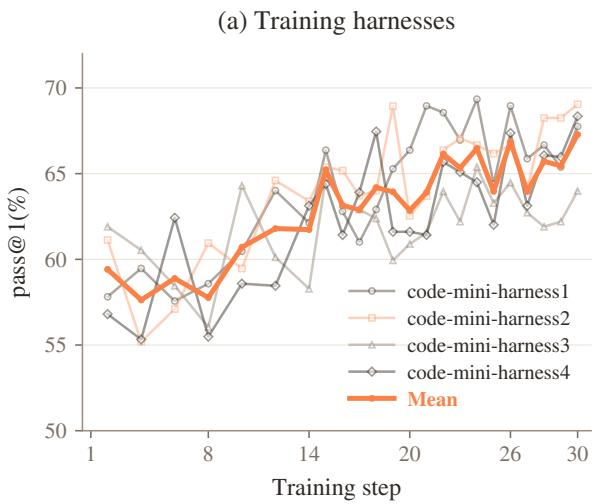
\includegraphics[keepaspectratio,alt={image}]{images/05afed0dc3b6a6ff8edb83fd1d2d8fbac26698d776f2005494d9fa7c2e54e4a2.jpg}}

\pandocbounded{\includegraphics[keepaspectratio,alt={image}]{images/ff08aa94c3d73433e9ba55fa657d1e623f888893f36a73da322aebc274e3600c.jpg}}

Figure 10 Pass@1 on DeepSWE v1.1 during Multi-Harness Training,
evaluated with (a) training harnesses and (b) held-out harnesses.
Lighter curves show individual harness results; thick orange curves show
the mean within each panel.

\subsection{5.4 Router Freezing for Stable
RL}\label{router-freezing-for-stable-rl}

Figure 11 compares two MiMo-V2.6-Pro RL runs that difer only in whether
the MoE router is frozen, tracking three expert-load statistics at
decoder layer 9: the coeficient of variation (CV), the peak load factor
(max/mean), and the fraction of cold experts below 0.1× the mean (loads
normalized per step). We observe a severe load-collapse problem when the
router is trainable: all three metrics rise monotonically over the first
20 steps, with CV increasing from 0.78 to 2.0, peak load from 6× to 16×,
and the cold-expert fraction from 0 5\% to 22\%. To diagnose the cause,
we restore the router parameters of the step-20 checkpoint to their
initial pre-RL values while keeping all other parameters unchanged: load
balance recovers to near-initial levels while benchmark performance
remains unchanged, indicating that the collapse is driven by router
drift rather than by degradation of the expert weights. We therefore
freeze the router for RL training; the frozen-router run keeps all three
statistics flat (CV ≈ 0.7, peak load ≈ 5.5×, cold fraction near 1\%)
with benchmark performance growing normally.

\subsection{5.5 RL Failure Analysis}\label{rl-failure-analysis}

Figure 12 summarizes interruptions in the MiMo-V2.6-Pro and
MiMo-V2.6-Flash training runs. Infrastructure failures were primarily
GPU-memory double-bit errors (DBEs). Flash was also restarted after a
Kubernetes failure caused pods in the Cyber-task cluster to crash
between steps 15 and 16. Pro was restarted after the grader became
unreachable over the network after step 14. Rollout failures arose in
the partial-rollout setting: shorter rollouts completed first after
startup, biasing length estimates in Predictive Rollout Dispatch (§6.3)
and exhausting both the GPU and pinned host-memory KV pools. Despite
early refinements, one harness later produced rollouts less than half as
long as those from other harnesses on the same code dataset, skewing
estimates in the second and third steps after restart. Training failures
were GPU out-of-memory (OOM) errors from MoE imbalance within a
micro-batch: at one layer, an expert-parallel (EP) rank received over
30× the mean token load despite a relatively balanced full batch. We
adjusted parallelism to reduce activation memory and accommodate these
peaks. Driverfailures occurred during packing late in Flash as longer
sequences increased per-node data volume beyond hostmemory capacity.
Although packing was distributed across nodes (§6.2), local memory
demand still caused CPU OOM and interrupted the run.

\pandocbounded{\includegraphics[keepaspectratio,alt={image}]{images/e3c12780901f591324c734c295079a553693582f5915c1c042107b372aef5172.jpg}}

\pandocbounded{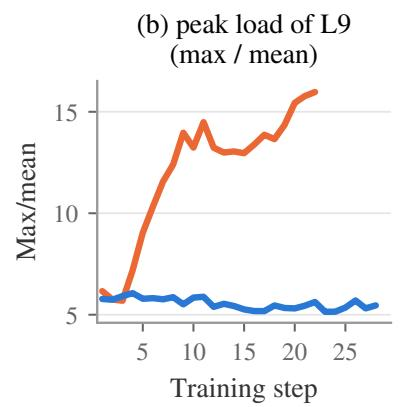
\includegraphics[keepaspectratio,alt={image}]{images/5977f57a82f575d068bf72798969d0d9f67e03dbcfa21527a5ee77bdcab624a7.jpg}}

\pandocbounded{\includegraphics[keepaspectratio,alt={image}]{images/4d80be3425e8b7d3835c3649acf6ee274d0268dcea8883a29a094c9aad309df0.jpg}}

Figure 11 MiMo-V2.6-Pro expert-load balance at decoder layer 9 (384
experts) during RL, comparing runs with and without freezing the router.
(a) Coeficient of variation of expert load. (b) Peak load factor
(max/mean). (c) Fraction of cold experts with load below 0.1× the mean.

\pandocbounded{\includegraphics[keepaspectratio,alt={image}]{images/2d158822d77be79047b5949312641d2371d72749b654df4ec35d722a575b6f38.jpg}}

Figure 12 MiMo-V2.6-Pro and MiMo-V2.6-Flash timelines over 30 training
steps, aligned by elapsed time. Light orange denotes completed steps;
other colors denote failure and recovery intervals by cause.

\subsection{5.6 Broadening Capabilities via
MOPD2}\label{broadening-capabilities-via-mopd2}

After mixed RL, we use Multi-Prefix Multi-Teacher On-Policy Distillation
(MOPD2) to combine capabilities from teachers trained for diferent
tasks, including tasks that are hard to verify. Building on MOPD from
MiMo-V2-Flash (Core Team et al., 2026; Ma et al., 2026), we retain
autonomous student rollouts in domains with suitable mixRL teachers
(Standard MOPD) and add prefix-conditioned single-turn rollouts (Liao et
al., 2026). Figure 13 illustrates the teacher configurations and the
standard and prefix-conditioned distillation workflows.

\begin{enumerate}
\def\labelenumi{(\alph{enumi})}
\tightlist
\item
  Domain-Specific Teachers
\end{enumerate}

\pandocbounded{\includegraphics[keepaspectratio,alt={image}]{images/6e55008df2ac9fe23013b1e6a04ca66eeef04291fbb058a6265c576b303aed60.jpg}}

Figure 13 Overview of MiMo MOPD2. (a) Domain-specialized teachers are
trained with MixRL on verifiable tasks or with SFT on synthetic
demonstrations for open-domain tasks. (b) Standard MOPD uses RL teachers
to supervise full student rollouts. (c) Prefix-Conditioned OPD reuses
trajectories from teacher rollouts (Teacher-Prefix OPD) or SFT data
(SFT-Prefix OPD). A source trajectory with � assistant-turn decision
points yields � complete history prefixes \(h _ { i } ,\) , each of
which can initialize a separate student-generated turn \(y _ { i }\) for
token-level distillation by the relevant domain teacher. SFT data
provide prefix contexts rather than fixed continuation targets.

Prefixes come from teacher rollouts (Teacher-Prefix OPD) or SFT data
(SFT-Prefix OPD). A trajectory with � assistant turns provides �
complete history prefixes, each ending before the corresponding turn.
The student samples one new turn from each prefix without regenerating
earlier interactions. A preassigned teacher provides token-level
supervision conditioned on the same history and the student's preceding
tokens.

For open-domain tasks where reliable RL rewards are dificult to design,
we train SFT teachers on high-quality synthetic demonstrations. Their
training may provide limited coverage of histories reached after
repeated student deviations in long-horizon tasks (Xu et al., 2025).
SFT-Prefix OPD therefore starts each rollout from a fixed demonstration
prefix, limiting deviations before the sam pled turn. Demonstrations
supply the context, while the student generates its own continuation
rather than imitating a fixed response.

MOPD2 further extends the capabilities of the RL-trained model to
domains where reliable trainingtime verification is challenging,
including those with complex environments or verifiers that are dificult
to design, such as long-horizon game development, scientific research,
and embodied intelligence. The final evaluation results of MiMo-V2.6 are
reported in Table 3. The MiMo-V2.6 series delivers substantial
improvements over MiMo-V2.5, achieving performance comparable to that of
frontier models across various domains.

{\def\LTcaptype{none} % do not increment counter
\begin{longtable}[]{@{}|l|l|l|l|l|l|l|@{}}
\toprule\noalign{}
\endhead
\bottomrule\noalign{}
\endlastfoot
\hline
Benchmark & MiMo-V2.6 Pro & MiMo-V2.6 Flash & MiMo-V2.5 Pro & Claude
Opus 5 & GPT-5.6 Sol & Claude Fable 5 \\
\hline
\multicolumn{7}{@{}l@{}}{%
Code Agent} \\
\hline
DeepSWE v1.1 & 71.9 & 67.9 & 19.0 & 74.0 & 73.0 & 70.0 \\
\hline
ProgramBench & 26.5 & 26.0 & 12.5 & 37.0 & 25.0 & 33.0 \\
\hline
MiMo Code Bench & 63.2 & 61.2 & 40.4 & 68.6 & 59.3 & - \\
\hline
\multicolumn{7}{@{}l@{}}{%
General Agent} \\
\hline
AutomationBench v1.0.6 & 53.1 & 52.3 & 16.0 & 50.3 & 45.8 & 46.2 \\
\hline
Toolathlon-Verified & 76.9 & 73.6 & 49.1 & 80.6 & 74.9 & 77.9 \\
\hline
GDPval-AA 2.1 & 1673 & - & 1107 & 1708 & 1588 & 1595 \\
\hline
Agents\textquotesingle{} Last Exam & 31.6 & 27.6 & 13.2 & 31.6 & 30.8 &
25.7 \\
\hline
Terminal Bench 4.0 & 34.9 & 28.8 & 1.5 & 49.0 & 39.9 & 42.4 \\
\hline
Terminal Bench 2.1 & 89.9 & 87.6 & 65.2 & 89.1 & 88.8 & 84.3 \\
\hline
OSWorld-Verified & 82.0 & 80.8 & - & 83.4 & 83.0 & 86.0 \\
\hline
JobBench & 62.0 & 61.2 & 25.0 & 65.7 & 45.4 & 57.4 \\
\hline
\multicolumn{7}{@{}l@{}}{%
Cybersecurity} \\
\hline
CyberGym & 94.0 & 95.1 & 40.0 & - & - & - \\
\hline
MiMo Cyber Bench & 80.2 & 77.2 & 0.0 & - & - & - \\
\hline
ExploitGym & 17.8 & 6.0 & 0.2 & 22.1 & 30.3 & 28.4 \\
\hline
ExploitBench & 47.9 & 25.3 & 16.6 & 70.0 & 78.5 & 78.0 \\
\hline
SEC Bench Pro & 66.3 & 47.5 & 17.7 & - & 79.1 & - \\
\hline
\multicolumn{7}{@{}l@{}}{%
Visual Agent} \\
\hline
MiMo Visual Coding & 72.3 & 71.5 & - & 70.0 & 73.4 & 69.1 \\
\hline
\end{longtable}
}

Table 3 Comparison of MiMo-V2.6 with previous-generation and frontier
models on agentic benchmarks.

\subsection{6 RL and OPD
Infrastructure}\label{rl-and-opd-infrastructure}

The MiMo-V2.6 series scales RL and OPD training to large mixed-task
batches of agentic rollouts. To support flexible agentic rollout
scenarios, we define the execution model and trajectory data structure,
and refine the learning signal with a Penalty Module (§6.1). At large
batch sizes, we implement the Harness Pool to host multiple harnesses
and sustain high rollout concurrency, and the Payload Porter to bufer
tens of thousands of trajectories heavy with routing and multimodal data
(§6.2). We implement a Sample Mixer that works with the dynamic sampler
and partial roll out to stably deliver training batches matching a
specified training distribution (§6.3). Towards stable and eficient RL
training, we align MoE routing and top-p sampling candidate sets between
the training and inference engines, while optimizing both engines for RL
workloads (§6.4).

\subsection{6.1 Agentic RL with Fine-grained Learning
Signals}\label{agentic-rl-with-fine-grained-learning-signals}

Agentic rollouts span multiple turns and dialogue contexts, while
outcome rewards provide only coarse supervision. We therefore adopt an
agent-centric execution model and organize trajectory data as a
hierarchy. Within this hierarchy, a configurable Penalty Module applies
loss masking and advantage shaping. It targets local model errors and
keeps infrastructure failures out of the training signal.

Agent Loop We shift rollout from an inference-centric design to an
agent-centric one: each sequence runs as an Agent Loop that owns the
environment lifecycle, manages the dialogues it produces, and calls the
inference engine on demand. The lifecycle covers setup, interaction,
reward evaluation (e.g., running test cases), and cleanup. During
interaction the loop exposes a request endpoint, and the external agent
drives the rollout by calling it. Each dialogue is kept both as a string
prefix and as a token sequence. Prefix matching locates the dialogue
that an incoming request extends, and only the new sufix is tokenized
and passed to the inference engine, keeping its interface purely
token-in, token-out.

Trajectory Hierarchy Subagents, context compaction, and multiple agent
roles produce concurrent dialogue branches within one rollout. We
organize the trajectory data into a four-level hierarchy: Sample →
Sequence → Context → Segment. A Sample is a prompt dispatched by the
Sample Mixer (§6.3). In group-wise algorithms such as GRPO (Shao et al.,
2024), the Sample spawns a group of Sequences, and the group is accepted
or rejected as a whole. A Sequence is one Agent Loop execution and may
contain several concurrent Contexts. A Context is one dialogue branch
holding a list of Segments; it is the unit of prefix matching, KV-cache
reuse, and trainingdata export. A Segment is a single turn---a system or
user message, a model generation, or a tool result---and only
model-generated turns contribute to the loss.

Penalty Module Group-wise algorithms spread the outcome reward evenly
across all modelgenerated tokens of a sequence. Within the hierarchy
above, credit is rarely uniform: some turns are of-path or degenerate,
and some failures are unrelated to the model. To assign credit where it
is due, we separate detection from its efect on training. A Rule judges
a segment, context, or sequence by handcrafted logic or a model-based
judge. For example, rules can catch infrastructure failures not
attributable to the model, garbled token patterns, calls to unavailable
tools, and repetition. A Strategy binds an action to a level of the
hierarchy: mask excludes the hit content from the loss, advantage
shaping sets, scales, or subtracts the advantages on hit tokens, and
monitor records metrics alone. The composite early stop strategy halts
the rollout as soon as its rule fires, zeroes the outcome reward,
applies separate actions to the triggering turn and earlier turns, and
masks sibling contexts. Penalties escalate along the hierarchy: a
context with no surviving model turns is dropped, a sequence with no
surviving context receives zero advantage, and a sample with no
surviving sequence is rejected. The specific penalties applied in
training are described in §4.3.3.

\subsection{6.2 Harness Pool and Payload Porter: Large-Batch RL with
Multiple
Harnesses}\label{harness-pool-and-payload-porter-large-batch-rl-with-multiple-harnesses}

Scaling RL training to large batches increases rollout concurrency and
the memory and commu nication costs of trajectory data. Mixed-task
batches add another axis of heterogeneity: a single batch mixes several
harnesses, with each training sample group bound to one harness. On the
execution side, the Harness Pool hosts concurrent harness instances and
Agent Loops in persistent multi-tenant actor pools, and harness
codebases, agent behavior, and environment settings are configured
independently. On the data side, the Payload Porter keeps the driver
scheduling on lightweight metadata alone. Heavy payloads are written
once to a distributed store and packed where they are consumed.
Multi-modal payloads split the same way into metadata and pixels, with
incremental transport and load-balanced encoding.

\pandocbounded{\includegraphics[keepaspectratio,alt={image}]{images/33ad1cd3d32005f7fea809508f5c6e7b84c71c92fdcc3ecb156104ba3d8f0d7d.jpg}}

Figure 14 Overview architecture of RL infrastructure.

Multi-tenant Rollout Execution We use Ray actors (Moritz et al., 2018)
to execute agent harnesses and Agent Loops across the cluster. A
dedicated Ray actor for every harness instance and Agent Loop would cost
one file descriptor per actor on Ray's global control store (GCS) node,
and a large batch would exhaust the GCS node's file descriptors. We
instead run fixed-size pools of persistent host actors, each carrying
many concurrent tenants---Agent Loops on the model side and harness
instances on the environment side. Each tenant keeps its own trajectory
state, and assignments are balanced by in-flight instance count. A host
is a single process whose tenants share one event loop. On the model
side they also share one request endpoint, one inference proxy, and one
tokenizer; on the environment side, one imported harness codebase. A
shared event loop would let one blocking call stall every tenant, so
blocking work---environment operations and tokenization---runs on
background threads. This amortizes process and service overhead across
concurrent rollouts, supporting larger concurrent batches without a
proportional increase in actor count.

Heterogeneous Agent Harnesses We configure harness codebases, agent
behavior, and environment settings separately to accommodate diverse
tasks within a single training run. Diferent data sources can use
diferent codebases, while agent configurations vary across prompts
within a source. Each training sample group uses a common configuration
for group-relative advantage estimation. One process can import only one
harness codebase, so diferent codebases run in separate pools. These
pools receive configurable shares of a fixed budget of host actors---set
once at startup, independent of the training-data mixture that is
scheduled every step. Harness diversity and rollout concurrency thus
scale within one execution framework.

Disaggregated Data Plane and Control Plane Scaled batches must bufer
tens of thousands of sequences at a time, and each is heavy: besides
token ids and log-probabilities, it carries MoE routing data, top-p
sampling indices, and multimodal data. Payload volume grows with both
sequence count and length, and gathering every payload on one driver
node ties batch size to that node's memory. We therefore disaggregate
the data plane from the control plane, splitting each sequence at
rollout finish: its payload is written once into a distributed key-value
store (e.g., the Ray object store or TransferQueue (Han et al., 2025)),
while the driver runs all scheduling on lightweight metadata---scalar
rewards, per-context lengths, and the keys addressing each payload. At
group finish, only the fields needed are read from the store: a few
columns for the accept-time hook. A group-wise grader, when configured,
runs fully asynchronously alongside the Agent Loops---its latency hidden
and its results free to lag---and rewrites the group rewards on return.
The sampler then accepts or rejects the group by passrate, on metadata
alone, and the hook imposes length penalties, computes group-relative
advantages, and applies advantage shaping. The per-token advantages are
written back into the store; groups whose advantages are all zero are
dropped by default. Under OPD, reward evaluation is replaced by teacher
scoring: each trajectory is sent to a teacher server, and its scores are
collected asynchronously into the same distributed store. At batch
yield---once each data source has contributed its share of the batch---a
yield hook packs the accepted sequences into micro-batches and assigns
them to ranks, touching no tensor. At pack time, one packer per training
tensor-parallel (TP) group serves every rank in the group. From the
unpadded rows in the store, it fetches only those its context-parallel
(CP) window touches and cuts out that window alone. The result is shared
across the TP group as a single read-only in-memory copy. This avoids
full-batch aggregation on the driver and dense padded intermediates
during packing.

Multi-Modal Data Multi-modal payloads follow the same meta/payload
split, but demand extra care: as the agent repeatedly takes screenshots
and reads images across turns, a single trajectory can accumulate
gigabytes of such data---costly to store, and costly to retransmit as
the history grows. During rollout, the Agent Loop therefore ships only
the multi-modal delta between requests (§6.4). For training, every image
item must pass through the vision encoder. Because the encoder is
replicated across the tensor-parallel group while the LLM backbone is
sharded, encoding runs data-parallel first---image items are balanced
across ranks independently of where each sequence's tokens land. After
encoding, embeddings are redistributed to the ranks holding the
corresponding tokens. The payload itself stays in the distributed
key-value store: load-balance planning reads only item metadata, and
pixels are fetched only for the encoder computation. This limits
redundant payload movement while accommodating uneven multi-modal
workloads.

\subsection{6.3 Sample Mixer: Stable Asynchronous Mixed-task
RL}\label{sample-mixer-stable-asynchronous-mixed-task-rl}

Since MiMo-V2-Flash (Core Team et al., 2026), we have maintained a Data
Scheduler that targets a specified training distribution across data
sources, together with dynamic sampler (Yu et al., 2025) and partial
rollout (Kimi Team, 2025). Mixed-task RL must preserve this distribution
de spite large variations in rollout duration and filtering rates, so
that every data source is trained efectively. Across 25 profiled data
sources, the mean generated tokens and the active rollout du ration vary
by 90× and 66×, respectively (Figure 15), motivating scheduling that
adapts to each source's workload. To meet these challenges, we implement
the Sample Mixer, with four mech anisms filling the specified training
distribution: Adaptive Rollout Concurrency sets per-source budgets,
Adaptive Rollout Scheduling selects data sources within the budgets,
Predictive Rollout Dispatch places new rollouts across ranks, and Sample
Replay covers startup and recovery.

Adaptive Rollout Concurrency Slower sources need more concurrent
rollouts to sustain the same training contribution. For source �, let
\(B _ { i }\) denote the target number of retained sample groups per
training step, \(r _ { i }\) the estimated group acceptance rate, and
\(t _ { i }\) the estimated active rollout duration, including model
generation and environment interaction but excluding pauses between
training steps. The expected generation demand is \$m \_ \{ i \} = \{ B
\_ \{ i \} \} / \{ r \_ \{ i \} \} ; \$ at a fixed training throughput,
the required concurrency scales with \(t _ { i } m _ { i }\) . We assign
each source a scheduling budget of \(( 1 + p _ { i } ) m _ { i }\)
groups, where the oversampling ratio \(p _ { i }\) satisfies

\pandocbounded{\includegraphics[keepaspectratio,alt={image}]{images/0c4c70693bd5b050a2a1b0e503c3bf1fb7462b2a0326d3806151b093523438cc.jpg}}

Mean generated tokens per rollout (thousands)

Figure 15 Rollout heterogeneity across 25 data sources. Each line
connects one source's Start point (faint) to its End point (solid); each
point plots that source's mean generated tokens against mean rollout
time over completed rollouts (tokens summed across dialogue contexts
before context filtering). Both axes are logarithmic.

\[
p _ {i} = \mathrm{clip} (c t _ {i} - 1, p _ {\min}, p _ {\max}), \qquad \frac {\sum_ {i} m _ {i} p _ {i}}{\sum_ {i} m _ {i}} = \bar {p}.\tag{6}
\]

The shared factor � keeps the demand-weighted mean of \(p _ { i }\) at
the global oversampling ratio \({ \bar { p } } ,\) subject to per-source
bounds. We recompute this allocation from recent timing and acceptance
statistics as workloads change. In steady state, the concurrency
requirement grows with a source's rollout duration and target, and falls
with its acceptance rate.

Adaptive Rollout Scheduling Within these budgets, scheduling balances
long-run generation demand with progress toward the current training
batch. If \(A _ { i }\) groups have already been accepted from source �
for the current batch, its scheduling weight is

\[
w _ {i} = \alpha \frac {B _ {i}}{r _ {i}} + (1 - \alpha) \frac {(B _ {i} - A _ {i}) ^ {+}}{r _ {i}},\tag{7}
\]

where \(( x ) ^ { + } = \operatorname* { m a x } ( x , 0 )\) and
\(\alpha \in [ 0 , 1 ]\) . The target term maintains generation demand;
the deficit term prioritizes sources with a remaining deficit. These
weights drive smooth weighted roundrobin; Steady-state startup combines
\(\alpha = 0 . 5\) with initial concurrency allocated in proportion to
\(t _ { i } m _ { i }\) . The trace-driven simulation in Figure 16
compares the policies at a fixed concurrency limit with nonbinding
source budgets: Deficit-corrected scheduling \(( \alpha = 0 . 5 )\)
improves occupancy stability over Deficit-based scheduling
\(\left( \alpha = 0 \right)\) and collection balance over Target-based
scheduling \(( \alpha = 1 )\) in this workload. Simulation durations are
calibrated to each source's mean rollout time at End in Figure 15.

Predictive Rollout Dispatch We jointly estimate KV demand and expected
inference concurrency to guide the admission and placement of new
rollouts across ranks. Per-source priors estimate a rollout's total
sequence length (input and generated tokens), summed across contexts;
these priors are updated from completed rollouts and used to estimate KV
demand. We admit a rollout only when a safety-margin multiple of its
estimated KV demand fits within the target rank's remaining GPU KV
capacity. Hierarchical caching (§6.4) spans HBM and a pinned host pool:
the two tiers jointly retain the state of admitted rollouts. The
estimated fraction of rollout time spent in environment execution
converts rollout concurrency into expected inference concurrency. We
bound this expectation by the max running requests used for CUDA graph
capture, limiting queueing delays that prolong rollout lifetimes and
increase staleness. To maximize throughput under both constraints, a
greedy heuristic selects the feasible rank with the greatest remaining
capacity---the minimum of available concurrency slots and remaining KV
capacity, both expressed in sequence units---with both quantities
updated after each placement.

\pandocbounded{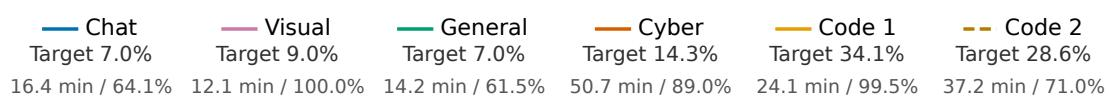
\includegraphics[keepaspectratio,alt={image}]{images/1ba3a9bfd797271372b1f73966603bb3e8b2f79459cfd294a93b75a51f023eff.jpg}}

\pandocbounded{\includegraphics[keepaspectratio,alt={image}]{images/a1b080c485a6a17ba18b27533b337ae385be5e195d307022610f5d25fbd5c961.jpg}}

Figure 16 Trace-driven scheduling simulation for six sources. Legend:
mean duration / group acceptance rate. Top: Collection progress
(accepted groups / nominal per-step targets, with surplus carried
forward). Bottom: Rollout occupancy (shares of occupied sequence slots).
Step spacing reflects elapsed time. Dotted lines mark step boundaries.
Training time, credit-assignment la tency, staleness expiry, and replay
are excluded.

Sample Replay We use sample replay to accelerate initial collection from
slow sources. In profiling, startup sample collection took approximately
1.8× as long as that of continuous operation. Within slow sources,
shorter rollouts tend to finish first, biasing the initial batch even
when persource targets are met. We therefore reuse completed rollout
groups from selected slow sources during the first collection step after
startup or checkpoint recovery, filling remaining per-source deficits
under current filtering rules. Fresh-start replay assumes that stored
rollouts were generated under the run's starting policy; recovery replay
reuses completed rollouts generated before recovery and still within
each source's staleness limit. Restricting replay to the first
collection step reduces the wait for slow sources while preserving the
specified training distribution.

\subsection{6.4 Training/Inference Consistency and
Optimization}\label{traininginference-consistency-and-optimization}

We extend the RL and OPD infrastructure of MiMo-V2-Flash (Core Team et
al., 2026), keeping SGLang (Zheng et al., 2024) and Megatron-LM (Shoeybi
et al., 2019) as the inference and the training engine, respectively. In
MiMo-V2.6, we use MXFP4 as the experts' data type during rollout. We
maintain alignment between the two engines in mixture-of-experts (MoE)
routing and probability normalization. On the inference side, the
Context Cache carries routing records, sampling candidate sets, and
visual inputs alongside the KV state across turns, and ofloads idle
state to host memory. A draft model trained on RL rollout logs further
accelerates generation through speculative decoding. On the training
side, we reduce the memory and communication costs of long sequences.

Training--Inference Consistency To support the MiMo-V2.6 series, we
apply quantize--dequantize (QDQ) to the experts after each parameter
update. The quantization follows the numeric con straints of the MXFP4
Humming GEMM kernels (vLLM Project, 2026) used during rollout, so the
two engines see identical expert weights. Even under identical
parameters, numerical diferences between the engines can flip discrete
expert selections; Rollout Routing Replay (R3) (Ma et al., 2025) records
the expert indices used during rollout and replays them during training,
reproducing the captured execution path. Top-k and top-p sampling
renormalize over a restricted candidate set rather than the full
vocabulary; we record each token's candidate set during rollout (Liu et
al., 2025a; The Microsoft AI Team, 2026) and renormalize the training
log-probabilities within it, matching the sampler's normalization. For
top-p sampling, only the GPU--CPU transfer is dense: we ship a bitmap of
fixed shape and full-vocabulary width. The fixed shape avoids a GPU--CPU
synchronization; the full width never truncates even a set that spans
the whole vocabulary. All later stages are sparse: at a typical top-p of
0.97, a candidate set averages fewer than five tokens. Both R3 and top-p
candidate-set replay incur negligible overhead, as the payloads stay
compact and move of the critical path.

Context Caching Following the request-level KVCache of MiMo-V2-Flash
(Core Team et al., 2026), each dialogue context has a persistent key:
within one policy version, later turns hit the cached KV---including
generated tokens---and prefill only the new sufix. Context caching is a
deliberately stateful choice: the cached state outlives each turn.
Expert indices and candi date sets are therefore not returned on
intermediate turns but only when the rollout is finally collected,
avoiding fragmented per-turn communication and processing. Historical
multimodal inputs need neither re-hashing nor re-sending: their visual
tokens already sit inside the cached KV. Only newly introduced images
cross the process boundary; full visual inputs are sent only after a
policy update or cache miss. Multi-turn environment interaction divides
a trajectory's wall clock into GPU time (generation) and tool time
(waiting on the environment); a hierarchical ex tension of the cache
reflects this temporal split spatially---a state resides in HBM during
GPU time and in a pinned host pool during tool time. Ofloading and
restoration run on side CUDA streams rather than the compute stream,
never stalling generation. HBM is thereby devoted to running requests as
far as possible: the larger the decode batch, the higher the arithmetic
intensity and compute utilization.

Draft Model Acceleration RL rollouts use block-6 DFlash for speculative
decoding by default, replacing the multi-token prediction (MTP-3)
configuration inherited from SFT. Initially trained on the SFT policy,
DFlash is then finetuned on early RL rollout logs resampled to match the
RL training distribution. Under this default configuration, average
accepted length is 31.3\% higher than with the MTP configuration. At
large RL batch sizes, we select the draft block size based on end-to-end
throughput rather than acceptance rate alone. Smaller draft blocks
reduce verification work: in mixed-task RL evaluation, block-6 improves
global average throughput by approximately 6\% over block-8, with little
change in average accepted length. Low-precision draft computation (FP8)
is also applied to reduce drafting overhead. On our long-context
workload, RL-adapted FP8 DFlash achieves approximately 10.3\% higher
per-node throughput than the baseline.

Training Optimization We train RL at a 1M-token context length.
MiMo-V2.6 interleaves 128- token sliding-window layers with full
attention. Under context parallelism, the sliding-window layers exchange
only the KV their queries can reach---at most a window-sized
segment---so perlayer trafic is bounded by the window rather than the
sequence length. Long sequences also inflate the memory footprint, and
MoE expert imbalance pushes peak memory higher. Optimizer states stay in
CPU memory and are copied back only for parameter updates. All loss
computation is fused into one kernel: the policy-gradient loss (with or
without top-p renormalization) and the OPD loss, optionally with metrics
such as entropy, label logit, and top-p mass. The fusion saves memory
and reduces step time.

\subsection{7 Open Foundations for Agentic
RL}\label{open-foundations-for-agentic-rl}

The MiMo-V2.6 series demonstrates the potential of reinforcement
learning to substantially advance agentic capabilities. Building on this
progress requires capable models and high-quality RL environments that
pair meaningful tasks with reliable verifiers. Sharing these resources
alongside reproducible baselines supports continued research and
innovation in the open-source community. We therefore open-source
MiMo-V2.6-Distill-Qwen-9B,2 a small model distilled from MiMo as a
shared starting point for further RL training. Alongside the model, we
release high-quality RL environments and an end-to-end open-source RL
framework. In this section, we establish domain-specific GRPO baselines
using these released resources. We also conduct a separate multi harness
training experiment using coding as a case study, following the approach
described for MiMo-V2.6. Our experiments show substantial gains across
multiple domains, demonstrating the value of these resources for RL
training.

\subsection{7.1 Distillation from
MiMo-V2.6}\label{distillation-from-mimo-v2.6}

Scaling RL computation and broadening the coverage of environments and
harnesses create more opportunities for exploration and learning. Across
these settings, efective exploration depends on coordinating actions and
responding to environmental feedback. Realizing the potential of agentic
RL therefore begins with a strong foundation of task-solving
capabilities.

To provide the open-source community with such a foundation, we develop
MiMo-V2.6-Distill-Qwen-9B by transferring MiMo's agentic experience into
a smaller model. We obtain the model by supervised fine-tuning
Qwen3.5-9B (Qwen Team, 2025) on MiMo-generated data spanning coding,
general-domain, visual, and cybersecurity tasks. The mixture contains
77.4 billion total tokens, including 27.2 billion loss tokens that
contribute to the SFT objective. Table 4 summarizes the data
composition.

The resulting MiMo-V2.6-Distill-Qwen-9B checkpoint improves over
Qwen3.5-9B across the reported evaluations (Table 6). For example,
SWE-bench Pro (Deng et al., 2025) increases from 32.0 to 44.6, and
AutomationBench from 5.0\% to 30.3\%. We view these strengthened
tasksolving capabilities as a promising foundation for further
improvement through RL. We therefore use this checkpoint as the common
initialization for the domain-specific GRPO experiments and the
multi-harness coding experiment described below.

{\def\LTcaptype{none} % do not increment counter
\begin{longtable}[]{@{}|l|l|l|l|@{}}
\toprule\noalign{}
\endhead
\bottomrule\noalign{}
\endlastfoot
\hline
Data source & Total tokens (B) & Token share (\%) & Loss tokens (B) \\
\hline
Code & 23.2 & 29.9 & 7.3 \\
\hline
Cyber & 11.0 & 14.2 & 4.8 \\
\hline
General & 22.0 & 28.5 & 5.7 \\
\hline
Visual & 21.2 & 27.4 & 9.4 \\
\hline
Total & 77.4 & 100.0 & 27.2 \\
\hline
\end{longtable}
}

Table 4 Weighted SFT data composition. Token counts are in billions.
Values are rounded to one decimal place; totals use unrounded aggregate
counts.

{\def\LTcaptype{none} % do not increment counter
\begin{longtable}[]{@{}|l|l|l|l|@{}}
\toprule\noalign{}
\endhead
\bottomrule\noalign{}
\endlastfoot
\hline
Domain & Task Family & Training Tasks & Verifier \\
\hline
Code & Software engineering & 3k & Executable tests \\
\hline
Cyber & Vulnerability reproduction & 1k & Rule checks \\
\hline
General & Knowledge work & 1k & Rubric-based judging \\
\hline
Visual & Web development & 2k & Visual grading \\
\hline
\end{longtable}
}

Table 5 Overview of the released RL environments, including training
task counts and the verifiers used to evaluate task completion. Task
counts are approximate, based on distinct task identifiers in each
training set; k denotes one thousand.

\subsection{7.2 RL with Open
Environments}\label{rl-with-open-environments}

Environments Overview Table 5 summarizes the RL environments we release
across coding, cybersecurity, general-domain, and visual tasks. The four
training sets contain approximately 7k tasks in total, with the
general-domain set focusing on knowledge work. The training resources
additionally include approximately 1k music-generation tasks, which
support the GRPO experi ments reported below.

RL Experiments Starting from the same MiMo-V2.6-Distill-Qwen-9B SFT
checkpoint, we conduct GRPO training separately for coding,
cybersecurity, general-domain, and visual tasks using the corresponding
released environments. Alongside public benchmarks, we evaluate on four
internal sets: MiMo Code Bench (mini) for software engineering , MiMo
Cyber Bench (mini) for vulnerability reproduction, MiMo General Bench
(mini) for knowledge work, and MiMo Visual Coding (mini) for website
development. These evaluation sets follow the same task distributions as
their corresponding training sets.

Table 6 shows that RL improves on the SFT checkpoint in all 11
evaluations reported in the table, spanning the four task domains.
SWE-bench Verified (Jimenez et al., 2024) rises from 61.1 to 66.2, while
Terminal Bench 2.1 (Merrill et al., 2026) improves from 37.1 to 52.8.
OficeQA Pro (Opsahl-Ong et al., 2026) improves from 19.5 to 24.8, and
Toolathlon-Verified (HKUST NLP, 2026) increases from 35.2 to 38.0. MiMo
Visual Coding (mini) improves from 64.0 to 72.4, and MiMo Cyber Bench
(mini) increases from 31.3 to 47.0. Beyond the tasks reported in Table
6, we also explore emerging tasks in artistic creation and design, such
as music composition. On our internal music benchmark, the score
improves substantially from 45.7 after SFT to 52.5 after RL.

{\def\LTcaptype{none} % do not increment counter
\begin{longtable}[]{@{}lllll@{}}
\toprule\noalign{}
\endhead
\bottomrule\noalign{}
\endlastfoot
\multirow{2}{*}{Benchmark} & \multirow{2}{*}{Metric} &
\multirow{2}{*}{Qwen3.5-9B} & \multicolumn{2}{l@{}}{%
MiMo-V2.6-Distill-Qwen-9B} \\
& & & SFT & RL \\
\multicolumn{5}{@{}l@{}}{%
Code} \\
SWE-bench Verified & avg@3 & 60.0 & 61.1 & 66.2 \\
SWE-bench Pro & avg@3 & 32.0 & 44.6 & 47.6 \\
MiMo Code Bench (mini) & avg@3 & 19.5 & 51.6 & 59.9 \\
\multicolumn{5}{@{}l@{}}{%
Cyber} \\
MiMo Cyber Bench (mini) & avg@3 & 5.7 & 31.3 & 47.0 \\
\multicolumn{5}{@{}l@{}}{%
General} \\
AutomationBench v1.0.6 & avg@1 & 5.0 & 30.3 & 33.1 \\
Terminal Bench 2.1 & avg@1 & 27.0 & 37.1 & 52.8 \\
Toolathlon-Verified & avg@1 & 25.9 & 35.2 & 38.0 \\
OfficeQA Pro & avg@1 & 9.0 & 19.5 & 24.8 \\
JobBench & avg@1 & 2.6 & 18.3 & 25.2 \\
MiMo General Bench (mini) & avg@1 & 28.5 & 62.2 & 70.6 \\
\multicolumn{5}{@{}l@{}}{%
Visual} \\
MiMo Visual Coding (mini) & avg@1 & 61.7 & 64.0 & 72.4 \\
\end{longtable}
}

Table 6 Evaluation of Qwen3.5-9B, MiMo-V2.6-Distill-Qwen-9B after SFT,
and the domainspecific checkpoints after further GRPO training (RL).
Code uses single-harness RL. The highest available score in each row is
bolded.

These results highlight the value of high-quality training data and a
strong SFT initialization for further improvement through RL.

Multi-Harness Training The coding results in Table 6 are obtained
through single-harness RL. We further investigate multi-harness training
in a separate coding experiment, starting from the same
MiMo-V2.6-Distill-Qwen-9B SFT checkpoint. Following the multi-harness
training approach described for MiMo-V2.6, we jointly optimize the model
across four mini-harnesses and evaluate it on these harnesses and three
additional held-out harnesses. Table 7 compares Qwen3.5-9B with
MiMo-V2.6-Distill-Qwen-9B before and after multi-harness RL across three
coding evalua tions and seven agent harnesses. MiMo-V2.6-Distill-Qwen-9B
improves on Qwen3.5-9B in all 21 dataset--harness pairs, and
multi-harness RL further improves every pair. On MiMo Code Bench (mini),
the additional gains over SFT range from 1.8 to 9.3 percentage points
across the seven harnesses.

Case Study To ofer a more intuitive view of how our SFT and RL recipe
progressively enhances model capabilities, we present a case study on
web development (a domain where visual quality is immediately apparent),
comparing websites generated by Qwen3.5-9B, MiMo-V2.6-Distill-Qwen-9B
(SFT), and MiMo-V2.6-Distill-Qwen-9B (RL) in Figure 17. As shown in the
left column, websites produced by Qwen3.5-9B appear relatively plain in
visual design, with simplistic layouts and minimal use of imagery.
Notably, the HR management interface in (c) sufers from clear layout
issues. After distillation, MiMo-V2.6-Distill-Qwen-9B (SFT) (middle
column) generates websites with noticeably richer content, more
harmonious color palettes, and more efective incorporation of image
assets, as exemplified by the photographic elements in the Ethiopia
heritage page in (b). Following RL training (right column), the model
takes a further step, delivering the most polished results with refined
typography, visually striking hero sections (e.g., the sunset imagery in
(b)), and more complete, well-structured page layouts (e.g., the fully
featured HR dashboard in (c) with sidebar navigation, a calendar widget,
and detailed statistics cards). These progressive qualitative
improvements align with the quantitative trajectory (61.7 → 64.0 → 72.4)
observed in Table 6, jointly demonstrating the cumulative benefits of
distillation from MiMo-V2.6 followed by RL in enhancing both the
aesthetic quality and functional completeness of generated outputs.

{\def\LTcaptype{none} % do not increment counter
\begin{longtable}[]{@{}lllllllll@{}}
\toprule\noalign{}
\endhead
\bottomrule\noalign{}
\endlastfoot
\multirow{2}{*}{Model} & \multicolumn{4}{l}{%
Training harnesses} & \multicolumn{3}{l}{%
Held-out harnesses} & \multirow{2}{*}{Mean} \\
& mini-harness1 & mini-harness2 & mini-harness3 & mini-harness4 & codex
& claude code & mini-swe-agent \\
\multicolumn{9}{@{}l@{}}{%
SWE-bench Verified} \\
Qwen3.5-9B & 58.4 & 36.4 & 54.8 & 57.8 & 48.6 & 54.8 & 60.6 & 53.1 \\
MiMo-V2.6-Distill-Qwen-9B & 61.7 & 63.9 & 61.7 & 63.1 & 58.5 & 61.7 &
65.3 & 62.3 \\
+ Multi-Harness RL & 67.9 & 65.1 & 66.6 & 67.2 & 61.1 & 65.3 & 66.7 &
65.7 \\
\multicolumn{9}{@{}l@{}}{%
SWE-bench Pro} \\
Qwen3.5-9B & 33.5 & 15.2 & 31.1 & 31.1 & 23.1 & 26.9 & 31.6 & 27.5 \\
MiMo-V2.6-Distill-Qwen-9B & 45.2 & 46.6 & 45.1 & 45.5 & 40.3 & 42.2 &
45.6 & 44.4 \\
+ Multi-Harness RL & 48.5 & 46.9 & 47.6 & 48.0 & 42.6 & 43.1 & 48.4 &
46.5 \\
\multicolumn{9}{@{}l@{}}{%
MiMo Code Bench (mini)} \\
Qwen3.5-9B & 19.0 & 7.5 & 16.5 & 22.5 & 10.5 & 13.5 & 17.5 & 15.3 \\
MiMo-V2.6-Distill-Qwen-9B & 53.2 & 56.7 & 51.5 & 56.3 & 46.0 & 51.2 &
56.8 & 53.1 \\
+ Multi-Harness RL & 62.5 & 64.5 & 57.0 & 63.3 & 50.7 & 53.0 & 62.0 &
59.0 \\
\end{longtable}
}

Table 7 Coding performance across agent harnesses. Mean is the
unweighted average of the seven harness scores, rounded to one decimal
place. The best result in each column within a dataset is bolded.

\subsection{8 Conclusion}\label{conclusion}

This report presents the MiMo-V2.6 series and a practical approach to
advancing foundation models through large-scale agentic reinforcement
learning. Building on an omni-capable foundation and agent-centric
mid-training, we scale RL along three dimensions: training batch size
and throughput, the diversity and complexity of environments and agent
harnesses, and the compute devoted to groupwise agentic grading. These
advances are supported by asynchronous training, mixed-task rollout
infrastructure, training--inference consistency mechanisms, and safe
guards against training drift and reward hacking. Together, they enable
sustained optimization over long-horizon interactions while improving
solution quality and token eficiency. Evaluations across public and
internal benchmarks demonstrate the efectiveness of this approach, with
MiMo-V2.6 achieving competitive performance against frontier models
across a broad range of agentic tasks.

To make this direction accessible to the research community, we release
MiMo-V2.6-Distill-Qwen-9B alongside curated task environments,
verifiers, an end-to-end RL framework, and composable mini-harnesses.
Consistent RL gains across domains and harnesses highlight the value of
these resources as a shared foundation for further experimentation. Our
work takes a practical step toward model self-improvement, emphasizing
the joint importance of broad exploration, informative feedback, and
scalable training systems. We hope these open resources support
reproducible research and cumulative progress toward increasingly
capable, general-purpose agents.

\begin{enumerate}
\def\labelenumi{(\alph{enumi})}
\tightlist
\item
  Can you build a software portfolio landing page called Momentum
  Software Studios?\ldots{} (truncated)
\end{enumerate}

\pandocbounded{\includegraphics[keepaspectratio,alt={image}]{images/d7d8c19d97c9c9b440be9d692895e0e792d3b4b265b758fa3b4ccf8e01577108.jpg}}

\pandocbounded{\includegraphics[keepaspectratio,alt={image}]{images/666b4d47f73df5c7747dc595a5fe6ace7a06ad02ce9fc6aff39dbc6adb7061f4.jpg}}

\pandocbounded{\includegraphics[keepaspectratio,alt={image}]{images/4ecf837255bb349137ab75c046b9aa8065d29969ed088923dd9bd1b3da5a130d.jpg}}

\begin{enumerate}
\def\labelenumi{(\alph{enumi})}
\setcounter{enumi}{1}
\tightlist
\item
  Can you build a website about the heritage of Ethiopia? Style: a warm
  palette of\ldots{} (truncated)
\end{enumerate}

\pandocbounded{
\includegraphics[keepaspectratio,alt={image}]{images/53fa55f4d8e781c346ea4d3b7d9d0f3b16dcb85ffb552890d1cf66b275159e8e.jpg}}

\begin{enumerate}
\def\labelenumi{(\alph{enumi})}
\setcounter{enumi}{2}
\tightlist
\item
  Create a modern HR Internship Management System interface with a white
  and light\ldots{} (truncated)
\end{enumerate}

\pandocbounded{\includegraphics[keepaspectratio,alt={image}]{images/8d04dc403054517589e21b9e584dacf1fe51e57d21985f093f7e9a9c3e848baf.jpg}}

Figure 17 Examples of website hero sections generated by Qwen3.5-9B,
MiMo-V2.6-Distill-Qwen-9B (SFT), and MiMo-V2.6-Distill-Qwen-9B (RL).
Each row (a--c) shows outputs from the three models for the same prompt.

\subsection{References}\label{references}

Artificial Analysis. GDPval-AA v2.1 Leaderboard, 2026. URL
https://artificialanalysis.ai/evalua tions/gdpval-aa. Accessed September
21, 2026.

I. Badertdinov, M. Nekrashevich, A. Shevtsov, and A. Golubev.
Swe-rebench v2: Languageagnostic swe task collection at scale, 2026. URL
https://arxiv.org/abs/2602.23866.

J. Chen, Y. Liang, and Z. Liu. Dflash: Block difusion for flash
speculative decoding, 2026. URL https://arxiv.org/abs/2602.06036.

Core Team, B. Xiao, B. Xia, B. Yang, B. Gao, B. Shen, C. Zhang, C. He,
C. Lou, F. Luo, et al.~MiMo-V2-Flash technical report, 2026. URL
https://arxiv.org/abs/2601.02780.

X. Deng, J. Da, E. Pan, Y. Y. He, C. Ide, K. Garg, N. Laufer, A. Park,
N. Pasari, C. Rane, et al.~Swe-bench pro: Can ai agents solve
long-horizon software engineering tasks?, 2025. URL
https://arxiv.org/abs/2509.16941.

F. Gloeckle, B. Y. Idrissi, B. Rozière, D. Lopez-Paz, and G. Synnaeve.
Better \& faster large language models via multi-token prediction. In
Forty-first International Conference on Machine Learning, ICML 2024,
Vienna, Austria, July 21-27, 2024. OpenReview.net, 2024. URL
https://openrevi ew.net/forum?id=pEWAcejiU2.

Z. Han, A. You, H. Wang, K. Luo, G. Yang, W. Shi, M. Chen, S. Zhang, Z.
Lan, C. Deng, et al.~Asyncflow: An asynchronous streaming rl framework
for eficient llm post-training, 2025. URL
https://arxiv.org/abs/2507.01663.

C. He, L. Li, S. Li, H. Lv, L. Kong, Q. Liu, T. Yang, and S. Ren.
Semantic head specialization guides hybrid vit attention for multimodal
llms, 2026. URL https://arxiv.org/abs/2608.28383.

HKUST NLP. Introducing Toolathlon-Verified, June 2026. URL
https://toolathlon.xyz/docs/bl og/toolathlon-verified.

W. Huang and P. Jiang. Deepswe v1.1: a cleaner, more reproducible
benchmark for frontier coding agents, 2026. URL
https://github.com/datacurve-ai/deep-swe.

W. Huang, C. Lee, L. Tng, and S. Ge. Deepswe: Measuring frontier coding
agents on original, long-horizon engineering tasks, 2026. URL
https://arxiv.org/abs/2607.07946.

C. E. Jimenez, J. Yang, A. Wettig, S. Yao, K. Pei, O. Press, and K. R.
Narasimhan. Swe-bench: Can language models resolve real-world github
issues? In The Twelfth International Conference on Learning
Representations, ICLR 2024, Vienna, Austria, May 7-11, 2024.
OpenReview.net, 2024. URL https://openreview.net/forum?id=VTF8yNQM66.

K. Jordan, Y. Jin, V. Boza, J. You, F. Cesista, L. Newhouse, and J.
Bernstein. Muon: An optimizer for hidden layers in neural networks,
2024. URL https://kellerjordan.github.io/posts/muon/.

Kimi Team. Kimi k1.5: Scaling reinforcement learning with llms, 2025.
URL https://arxiv.org/ abs/2501.12599.

H. Lee, J. Liu, D. Kim, Z. Zhang, C. S. Xia, and L. Zhang. Sec-bench
pro: Can language models solve long-horizon software security tasks?,
2026. URL https://arxiv.org/abs/2605.26548.

S. Lee and D. Brumley. Exploitbench: A capability ladder benchmark for
LLM cybersecurity agents, 2026. URL https://arxiv.org/abs/2605.14153.

J. Li, W. Zhao, J. Zhao, W. Zeng, H. Wu, X. Wang, R. Ge, Y. Cao, Y.
Huang, W. Liu, J. Liu, Z. Su, Y. Guo, F. Zhou, L. Zhang, J. Michelini,
X. Wang, X. Yue, S. Zhou, G. Neubig, and J. He. The tool decathlon:
Benchmarking language agents for diverse, realistic, and long-horizon
task execution. In International Conference on Learning Representations,
2026a. URL https://ar xiv.org/abs/2510.25726.

Y. Li, Y. Feng, Z. Xu, Z. Ma, K. Zheng, F. Jiang, X. Sun, R. Shao, Z.
Chen, Y. Huang, X. Han, B. Lee, K. Xu, S. Zeng, H. Hua, X. Zhang, B.
Alomair, R. Krishna, L. Zettlemoyer, P. W. Koh, B. Ramasubramanian, L.
Niu, X. Yue, and R. Poovendran. JobBench: Aligning agent work with human
will, 2026b. URL https://arxiv.org/abs/2605.26329.

B. Liao, H. Dong, C. Monz, X. Xu, L. Dong, and F. Wei. Multi-turn
on-policy distillation with prefix replay, 2026. URL
https://arxiv.org/abs/2607.04763.

K. Lion, F. Hübler, B. Li, A. Orvieto, and N. He. Muown: Row-norm
control for Muon optimization, 2026. URL
https://arxiv.org/abs/2605.10797.

A. Liu, B. Feng, B. Xue, B. Wang, B. Wu, C. Lu, C. Zhao, C. Deng, C.
Zhang, C. Ruan, et al.~Deepseek-v3 technical report, 2024. URL
https://arxiv.org/abs/2412.19437.

A. Liu, A. Mei, B. Lin, B. Xue, B. Wang, B. Xu, B. Wu, B. Zhang, C. Lin,
C. Dong, et al.~Deepseekv3.2: Pushing the frontier of open large
language models, 2025a. URL https://arxiv.org/abs/ 2512.02556.

J. Liu, J. Su, X. Yao, Z. Jiang, G. Lai, Y. Du, Y. Qin, W. Xu, E. Lu, J.
Yan, Y. Chen, H. Zheng, Y. Liu, S. Liu, B. Yin, W. He, H. Zhu, Y. Wang,
J. Wang, M. Dong, Z. Zhang, Y. Kang, H. Zhang, X. Xu, Y. Zhang, Y. Wu,
X. Zhou, and Z. Yang. Muon is scalable for LLM training, 2025b. URL
https://arxiv.org/abs/2502.16982.

W. Ma, H. Zhang, L. Zhao, Y. Song, Y. Wang, Z. Sui, and F. Luo.
Stabilizing moe reinforcement learning by aligning training and
inference routers, 2025. URL https://arxiv.org/abs/2510.1 1370.

W. Ma, J. Wei, L. Zhao, H. Zhang, B. Xiao, L. Li, Q. Yang, B. Gao, Y.
Wang, R. Li, J. Dong, Z. Sui, and F. Luo. Mopd: Multi-teacher on-policy
distillation for capability integration in llm posttraining, 2026. URL
https://arxiv.org/abs/2606.30406.

R. Marten, A. Shaw, I. Bercovich, B. Droste, T. Cerruti, S. Dillmann, R.
Wang, D. Wahdany, A. Hart, K. Krauth, ScaleAI, Snorkel AI, Turing,
gNucleus AI, Boolean AI, N. Carlini, S. Lyu, A. Wei, A. Khatua, B.
Plüster, C. Dwivedi, C. Sutclife, Yuming, D. Tivris, D. Wang, H. W. Goh,
H. Xing, H. Lin, I. Salia, J. Seol, J. Bao, J. Ouyang, J. Park, L.
Walsh, L. Kong, M. Ivanov, M. Ubl, M. Liamets, O. Menis, P. Migdal, Q.
Bao, R. Movva, R. Ben Chaim, N. Srinath, S. Bog danik, S. Yadav, S.
Benjamin, T. Kung, W. Hughes, X. Lan, H. Gupta, S. Mishra, C. Wang, H.
He, J. Tu, K. Montgomery, Z. Tu, A. Naik, D. Mortensen, I. Zhang, Y.
Mathur, E. Liu, K. Singh, M. Yu, S. Feng, V. Gangal, Z. Tao, S. Ruan, J.
Mueller, J. Cabezas, J. Bauer, K. X. Li, R. Zhang, A. Feller, A.
Madayan, L. Chen, B. Feuer, X. Li, B. Li, H. Raj, S. Galler, L. Shi, I.
Segal, K. Buchanan, S. P., R. Desai, A. Schneider, C. Settles, X. Lin,
M. Nezhurina, A. Wang, M. Kowalczyk, J.-X. Zhao, S. Satia, J. Hu, S.
Atef, K. Chen, S. Vance, G. Segato, J. Jitsev, A. Dimakis, M. Merrill,
A. Konwinski, and L. Schmidt. Terminal-Bench, 2026. URL
https://github.com/harbor-framework/terminal-bench/releases/tag/v4.0.0.
Software release, version 4.0.0.

M. A. Merrill, A. G. Shaw, N. Carlini, B. Li, H. Raj, I. Bercovich, L.
Shi, J. Y. Shin, T. Walshe, E. K. Buchanan, J. Shen, G. Ye, H. Lin, J.
Poulos, M. Wang, M. Nezhurina, J. Jitsev, D. Lu, O. M. Mastromichalakis,
Z. Xu, Z. Chen, Y. Liu, R. Zhang, L. L. Chen, A. Kashyap, J.-L. Uslu, J.
Li, J. Wu, M. Yan, S. Bian, V. Sharma, K. Sun, S. Dillmann, A. Anand, A.
Lanpouthakoun, B. Koopah, C. Hu, E. Guha, G. H. S. Dreiman, J. Zhu, K.
Krauth, L. Zhong, N. Muennighof, R. Amanfu, S. Tan, S. Pimpalgaonkar, T.
Aggarwal, X. Lin, X. Lan, X. Zhao, Y. Liang, Y. Wang, Z. Wang, C. Zhou,
D. Heineman, H. Liu, H. Trivedi, J. Yang, J. Lin, M. Shetty, M. Yang, N.
Omi, N. Raoof, S. Li, T. Y. Zhuo, W. Lin, Y. Dai, Y. Wang, W. Chai, S.
Zhou, D. Wahdany, Z. She, J. Hu, Z. Dong, Y. Zhu, S. Cui, A. Saiyed, A.
Kolbeinsson, J. Hu, C. M. Rytting, R. Marten, Y. Wang, A. Dimakis, A.
Konwinski, and L. Schmidt. Terminal-Bench: Benchmarking agents on hard,
realistic tasks in command line interfaces, 2026. URL
https://arxiv.org/abs/2601.11868.

P. Moritz, R. Nishihara, S. Wang, A. Tumanov, R. Liaw, E. Liang, M.
Elibol, Z. Yang, W. Paul, M. I. Jordan, et al.~Ray: A distributed
framework for emerging \{AI\} applications. In 13th USENIX symposium on
operating systems design and implementation (OSDI 18), pages 561--577,
2018.

K. Opsahl-Ong, A. Singhvi, J. Collins, I. Zhou, C. Wang, A. Baheti, O.
Oertell, J. Portes, S. Havens, E. Elsen, M. Bendersky, M. Zaharia, and
X. Chen. Oficeqa pro: An enterprise benchmark for end-to-end grounded
reasoning, 2026. URL https://arxiv.org/abs/2603.08655.

T. Patwardhan, R. Dias, E. Proehl, G. Kim, M. Wang, O. Watkins, S. P.
Fishman, M. Aljubeh, P. Thacker, L. Fauconnet, N. S. Kim, P. Chao, S.
Miserendino, G. Chabot, D. Li, M. Sharman, A. Barr, A. Glaese, and J.
Tworek. GDPval: Evaluating AI model performance on real-world
economically valuable tasks, 2025. URL https://arxiv.org/abs/2510.04374.

PrimeIntellect. Swe-rl: Software engineering tasks for rl, 2026. URL
https://huggingface.co/col lections/PrimeIntellect/swe-rl.

X. Qu, P. Huang, and S. Horvath. Can Muon fine-tune Adam-pretrained
models?, 2026. URL https://arxiv.org/abs/2605.10468.

Qwen Team. Qwen3-next: Towards ultimate training \& inference eficiency.
https://qwen.ai/blog
?id=4074cca80393150c248e508aa62983f9cb7d27cd\&from=research.latest-advancements-list,
September 2025.

I. Shah, A. M. Polloreno, K. Stratos, P. Monk, A. Chaluvaraju, A. Hojel,
A. Ma, A. Thomas, A. Tanwer, D. J. Shah, K. Nguyen, K. Smith, M.
Callahan, M. Pust, M. Parmar, P. Rushton, P. Mazarakis, R. Kapila, S.
Srivastava, S. Singla, T. Romanski, Y. Vanjani, and A. Vaswani.
Practical eficiency of Muon for pretraining, 2025. URL
https://arxiv.org/abs/2505.02222.

Z. Shao, P. Wang, Q. Zhu, R. Xu, J. Song, X. Bi, H. Zhang, M. Zhang, Y.
K. Li, Y. Wu, and D. Guo. Deepseekmath: Pushing the limits of
mathematical reasoning in open language models, 2024. URL
https://arxiv.org/abs/2402.03300.

D. Shepard and R. Salimans. AutomationBench, 2026. URL
https://arxiv.org/abs/2604.18934.

M. Shoeybi, M. Patwary, R. Puri, P. LeGresley, J. Casper, and B.
Catanzaro. Megatron-lm: Training multi-billion parameter language models
using model parallelism, 2019. URL https://arxiv. org/abs/1909.08053.

Y. Sun, X. Han, W. Zhang, Y. Pang, T. Wang, Y. Cao, Y. Huang, C. Duroiu,
H. Zhang, J. Lin, W. Zhang, T. Zeng, Y. Yan, B. Liu, H. Wen, M. Xu, X.
Liu, Z. Chen, W. Shi, A. Dsouza, V. S. Chen, P. Bryant, C. Boettiger, Y.
Rangan, B. Rothenberg, K. Steinfeld, A. Rao, T. Schneider, G.
Yannakakis, L. Zanna, K. Ozbay, I. Sim, T. Zohdi, G. E. Karniadakis, J.
Gallant, T. Head-Gordon, Y. Li, W. Deng, T. Sun, H. Wang, Z. Wang, J.
Xu, C. Y. Liu, Y. Cheng, R. Hu, A. Bacho, S. Cao, Z. Qin, Y. Chen, H.
Fan, H. Liu, L. Zeng, S. M. Bharadwaj, L. Gong, Y. Yang, M. Song, R.
Wang, Z. Zhang, H. Bao, S. Lu, J. Tu, Z. Wang, Z. Zhang, Z. Chen, Y.
Jiang, Z. Li, B. Lyu, C. Ma, P. Xu, B. Zhang, S. Gu, H. Hua, H. Li, W.
Liao, C. Liu, J. Peng, H. Sun, Z. Xu, B. Chen, J. Cheng, Y. Jiang, K.
Kuang, Y. Li, Y. Pan, Z. Rao, A. Schubert, Y. Shen, V. Siu, X. Sun, K.
Zhang, X. Zhang, Y. Zhu, I. S. Chandok, L. Ding, J. Fan, A. Glover, J.
Hu, Y. Hu, W. Huang, Z. Jiang, H. Jin, L. Kim, M. Liu, Y. Liu, A.
Rafiei, X. Shen, K. Sun, S. Sun, T. Sun, E. Wang, Y. Wang, H. Xing, S.
Xu, Y. Xu, Z. Xu, Z. Yan, B. Yuan, R. Zhang, Y. Zhang, Z. Zhao, Liana,
S. B. Antu, H. Bai, C. Bosio, J. Cavanagh, P. Cavazos-Rehg, T. Chen, X.
Chen, Y. Chen, C. Zhu, C. Dai, S. D. Castro, Y. Deng, K. Dhole, J. Ding,
C. Du, Z. Du, H. Fan, R.-Z. Fan, H. Fu, S. Gu, Y. Gu, C. Guo, B. Huang,
B. Huang, R. Jaiswal, Z. Jiang, R. Jin, E. Kasson, X. Lan, J. Lee, D.
Lei, C. Li, D. Li, H. Li, H. Li, J. Li, X. Li, Y. Li, Y. Li, Y. Li, Z.
Li, W. Liang, L. Liao, K. Q. Lin, A. Z. Liu, C. Liu, J. Liu, K. Liu, X.
Liu, P. Lu, W. Lv, Y. Lyu, Q. Mang, K. Montgomery, Y. Nie, R. Ning, J.
Overwiening, X. Pan, L. Paraboschi, C. F. Park, J. Purnomo, S. Rajwal,
S. Rankin, B. Ren, Y. Rong, H. Shang, V. Shaw, F. Shen, J. Shen, M. Shi,
S. Qiu, H. Yao, T. Shi, J. So, V. Susoy, H. Szlyk, H. Wang,

J. Wang, W. Wang, X. Wang, Z. Wang, D. Wong, A. Wu, D. Wu, F. Wu, M. M.
Wu, Y. Wu, Y. Wu, Y. Wu, Q. Wuwu, W. Xiao, Y. Xiong, F. Xu, R. Xu, M.
Yan, B. Yang, J. Yang, S. Yang, X. Yang, Y. Yang, H. Ye, X. Yu, Z. Yu,
C. Zhang, C. Zhang, H. Zhang, H. Zhang, J. Zhang, K. Zhang, S. Zhang, W.
Zhang, W. Zhang, Y. Zhang, Y. Zhang, B. Zhao, Q. Zhao, Y. Zhao, Y.
Zheng, L. Zhou, T. Zhou, S. Zhu, S. Zhu, Y. Zhu, Y. Zhu, J. Zuo, C. Cai,
H. Casademunt, W. Chen, C. Cheng, N. Deng, R. Fu, T. Fu, Y. Han, H. Ren,
Z. He, Q. Jin, L. Li, Y. Li, S. Liu, L. Lu, L. Zhou, S. Mukherjee, Y.
Ouyang, Y. Ren, D. Shi, H. Wu, Z. Wu, H. Yao, Z. Yi, J. Yu, R. Zhan, H.
Zhou, B. Zhu, J. Zhu, A. Yuille, Y. Liu, R. A. Poldrack, J. Li, Z. Li,
M. Tao, J. Huang, W. Shi, C. Spanos, L. Sun, C. Wang, O. Xu, Z. Dong, H.
Gomez, A. Caliskan, A. Emami, H. Hu, Z. Li, L. Liu, M. Niu, Y. Shao, J.
Sun, M. Tolonen, T. Wang, S. Das, Y. Gao, W. Guo, E. J. Schneider, Z.
Lu, Y. Ma, M. Mueller, R. Poovendran, S. Sojoudi, Y. Zhu, and D. Song.
Agents' last exam, 2026. URL https://arxiv.org/abs/2606.05405.

C. Tao, J. Chen, Y. Jiang, K. Kou, S. Wang, R. Wang, X. Li, S. Yang, Y.
Du, J. Dai, Z. Mao, X. Wang, L. Shang, and H. Bai. Swe-lego: Pushing the
limits of supervised fine-tuning for software issue resolving, 2026. URL
https://arxiv.org/abs/2601.01426.

The Microsoft AI Team. MAI-Thinking-1: Building a hill-climbing machine.
Technical report, Microsoft AI, 2026. URL
https://microsoft.ai/pdf/mai-thinking-1.pdf.

A. Vaswani, N. Shazeer, N. Parmar, J. Uszkoreit, L. Jones, A. N. Gomez,
L. Kaiser, and I. Polosukhin. Attention is all you need. In I. Guyon, U.
von Luxburg, S. Bengio, H. M. Wallach, R. Fergus, S. V. N. Vishwanathan,
and R. Garnett, editors, Advances in Neural Information Processing
Systems 30: Annual Conference on Neural Information Processing Systems
2017, December 4-9, 2017, Long Beach, CA, USA, pages 5998--6008, 2017.
URL https://proceedings.neurips.
cc/paper/2017/hash/3f5ee243547dee91fbd053c1c4a845aa-Abstract.html.

vLLM Project. Humming. h t t p s : / / g i t h u b . c o m / v l l m- p
r oj e c t / h u m m i n g / r e l e a s e s / t a g / v 0 . 1 . 1 5,
September 2026. Version 0.1.15, GitHub repository, commit
a74973b5079e42ef861720b62f847ce9d33447f5; accessed 2026-09-19.

Z. Wang, T. Shi, J. He, M. Cai, J. Zhang, and D. Song. Cybergym:
Evaluating AI agents' cybersecurity capabilities with real-world
vulnerabilities at scale, 2025. URL https://arxiv.org/abs/ 2506.02548.

Z. Wang, N. Schiller, H. Li, S. S. Narayana, M. Nasr, N. Carlini, X. Qi,
E. Wallace, E. Bursztein, L. Invernizzi, K. Thomas, Y. Shoshitaishvili,
W. Guo, J. He, T. Holz, and D. Song. Exploitgym: Can AI agents turn
security vulnerabilities into real attacks?, 2026. URL
https://arxiv.org/ab s/2605.11086.

B. Xia, B. Shen, D. Zhu, D. Zhang, G. Wang, H. Zhang, H. Liu, J. Xiao,
J. Dong, L. Zhao, et al.~Mimo: Unlocking the reasoning potential of
language model--from pretraining to posttraining, 2025. URL
https://arxiv.org/abs/2505.07608.

L. Xiaomi. Mimo-audio: Audio language models are few-shot learners,
2025. URL https://arxiv. org/abs/2512.23808.

T. Xie, D. Zhang, J. Chen, X. Li, S. Zhao, R. Cao, T. J. Hua, Z. Cheng,
D. Shin, F. Lei, Y. Liu, Y. Xu, S. Zhou, S. Savarese, C. Xiong, V.
Zhong, and T. Yu. Osworld: Benchmarking multimodal agents for open-ended
tasks in real computer environments. In A. Globersons, L. Mackey, D.
Belgrave, A. Fan, U. Paquet, J. M. Tomczak, and C. Zhang, editors,
Advances in Neural Information Processing Systems 37: Annual Conference
on Neural Information Processing Systems 2024, NeurIPS 2024, Vancouver,
BC, Canada, December 10 - 15, 2024, 2024. doi: 10.52202/07901

7-1650. URL
http://papers.nips.cc/paper\_files/paper/2024/hash/5d413e48f84dc61244b6be5
50f1cd8f5-Abstract-Datasets\_and\_Benchmarks\_Track.html.

XLANG Lab. Introducing OSWorld-Verified, July 2025. URL
https://xlang.ai/blog/osworld-verif ied.

W. Xu, R. Han, Z. Wang, L. T. Le, D. Madeka, L. Li, W. Y. Wang, R.
Agarwal, C. Lee, and T. Pfister. Speculative knowledge distillation:
Bridging the teacher-student gap through interleaved sampling. In The
Thirteenth International Conference on Learning Representations, ICLR
2025, Singapore, April 24-28, 2025. OpenReview.net, 2025. URL
https://openreview.net/forum?i d=EgJhwYR2tB.

J. Yang, K. Lieret, J. Ma, P. Thakkar, D. Pedchenko, S. Sootla, E.
McMilin, P. Yin, R. Hou, G. Synnaeve, D. Yang, and O. Press.
Programbench: Can language models rebuild programs from scratch?, 2026a.
URL https://arxiv.org/abs/2605.03546.

S. Yang, C. Tao, J. Chen, T. Yu, R. Wang, Y. Jiang, Y. Du, W. Xu, J.
Xiong, T. Wu, L. Shang, X. Li, N. Wong, and H. Bai. What makes
interaction trajectories efective for training terminal agents?, 2026b.
URL https://arxiv.org/abs/2606.03461.

B. Ye, L. Li, S. Li, Z. Yue, L. Zhang, H. Lv, Y. Liu, W. Ma, H. Tian, R.
Li, J. Dong, Y. Zhao, X. Deng, H. Zhang, L. Zhao, Q. Liu, L. Kong, T.
Yang, and F. Luo. CodeMidas: Scaling agentic coding rl environments from
code itself, 2026. URL https://arxiv.org/abs/2609.22068.

Q. Yu, Z. Zhang, R. Zhu, Y. Yuan, X. Zuo, Y. Yue, W. Dai, T. Fan, G.
Liu, J. Liu, L. Liu, X. Liu, H. Lin, Z. Lin, B. Ma, G. Sheng, Y. Tong,
C. Zhang, M. Zhang, R. Zhang, W. Zhang, H. Zhu, J. Zhu, J. Chen, J.
Chen, C. Wang, H. Yu, Y. Song, X. Wei, H. Zhou, J. Liu, W. Ma, Y. Zhang,
L. Yan, Y. Wu, and M. Wang. DAPO: an open-source LLM reinforcement
learning system at scale. In D. Belgrave, C. Zhang, L. N. Montoya, H.
Lin, R. Pascanu, P. Koniusz, M. Ghassemi, N. Chen, I. V. M. Ruíz, and A.
Loaiza-Bonilla, editors, Advances in Neural Information Processing
Systems 38: Annual Conference on Neural Information Processing Systems
2025, NeurIPS 2025, San Diego, CA, USA, December 2-7, 2025 / Mexico
City, Mexico, November 30 - December 5, 2025, 2025. URL
http://papers.nips.cc/paper\_files/paper/2025/hash/a4277
440d50f1f15d2cb4c14f7e0c0d2-Abstract-Conference.html.

Z. Yue, Z. Lin, Y. Song, W. Wang, S. Ren, S. Gu, S. Li, P. Li, L. Zhao,
L. Li, et al.~Mimo-vl technical report, 2025. URL
https://arxiv.org/abs/2506.03569.

D. Zan, Z. Huang, W. Liu, H. Chen, S. Xin, L. Zhang, Q. Liu, A. Li, L.
Chen, X. Zhong, S. Liu, Y. Xiao, L. Chen, Y. Zhang, J. Su, T. Liu, R.
Long, M. Ding, and L. Xiang. Multi-swebench: A multilingual benchmark
for issue resolving. In D. Belgrave, C. Zhang, L. N. Montoya, H. Lin, R.
Pascanu, P. Koniusz, M. Ghassemi, N. Chen, I. V. M. Ruíz, and A.
Loaiza-Bonilla, editors, Advances in Neural Information Processing
Systems 38: Annual Conference on Neural Information Processing Systems
2025, NeurIPS 2025, San Diego, CA, USA, December 2-7, 2025 / Mexico
City, Mexico, November 30 - December 5, 2025, 2025. URL http:
//papers.nips.cc/paper\_files/paper/2025/hash/5afa9cb1e917b898ad418216dc726fbd-A
bstract-Datasets\_and\_Benchmarks\_Track.html.

J. Zhao, G. Chen, F. Meng, M. Li, J. Chen, H. Xu, Y. Sun, X. Zhao, R.
Song, Y. Zhang, P. Wang, C. Chen, J. Wen, and K. Jia. Immersion in the
github universe: Scaling coding agents to mastery, 2026. URL
https://arxiv.org/abs/2602.09892.

L. Zheng, L. Yin, Z. Xie, C. Sun, J. Huang, C. H. Yu, S. Cao, C.
Kozyrakis, I. Stoica, J. E. Gonzalez, C. W. Barrett, and Y. Sheng.
Sglang: Eficient execution of structured language model programs. In A.
Globersons, L. Mackey, D. Belgrave, A. Fan, U. Paquet, J. M. Tomczak,
and C. Zhang, editors, Advances in Neural Information Processing Systems
37: Annual Conference on Neural Information Processing Systems 2024,
NeurIPS 2024, Vancouver, BC, Canada, December 10 - 15, 2024, 2024. URL
http://papers.nips.cc/paper\_files/paper/2024/hash/724be4472168f31
ba1c9ac630f15dec8-Abstract-Conference.html.

\subsection{A Contributions and
Acknowledgments}\label{a-contributions-and-acknowledgments}

We would like to express our sincere gratitude to all contributors for
their invaluable support and eforts, including the Xiaomi Data Platform,
CloudML, NGK, MiChat, Mify, MiKS and LLM-Plus teams, as well as those
not explicitly listed in this paper. Within each role, authors are
listed in reverse alphabetical order by first name.

Core Contributors: Zongming Qiao, Ziyue Hua, Zirui Ou, Zihao Yue, Zihan
Jiang, Zhuo Huang, Zhiyang Chen, Zhixian Zheng, Zhipeng Xu, Zhengrui Ma,
Yuyang Hu, Yuhang Dong, Yuechen Zhang, Yudong Wang, Yuanxin Liu, Yixin
Yang, Yishuo Cai, Yikai Zhao, Yihan Yan, Yifan Zhang, Yifan Song, Xiyu
Wei, Xing Zhang, Xin Zhang, Xiaoqian Liu, Xiaodong Ji, Xiangwei Deng,
Xueyu Guo, Wenhan Ma, Weimin Xiong, Weikun Wang, Weiji Zhuang, Shuo Liu,
Shuhuai Ren, Shuhao Gu, Shimao Chen, Shijie Cao, Shihua Yu, Shicheng Li,
Shengjie Zhou, Shaolei Zhang, Rang Li, Qiying Wang, Qingkai Fang, Qianli
Chen, Minzheng Wang, Liwen Wang, Linli Yao, Linghao Zhang, Liangyu
Cheng, Liang Zhao, Lei Li, Jinhao Dong, Jinyu Xiang, Jianyu Wei,
Jiangshan Duo, Huaqiu Liu, Huanjie Fan, Hongyi Guan, Hongshen Xu, Hao
Tian, Hanyu Li, Hailin Zhang, Gang Wang, Fuli Luo†, Feng Wei, Dong
Zhang, Dawei Zhu, Chiheng Lou, Chenhong He, Chenhao He, Chenghua Liu,
Bowen Ye, Bowen Shen, Boshen Xu, Bo Yang, Bingquan Xia, Bangjun Xiao,
Baixuan Xu

Contributors: Zhouxiang Mao, Zhiyang Zhang, Zhixiang Xu, Zhenru Lin,
Zhengju Tang, Zhaojun Huang, Yuzhe Weng, Yuxing Xiang, Yuxiao Li, Yuheng
Yang, Yuhang Wang, Yuchen Liu, Yuanyuan Tian, Yuanliang Dong, Yu Cheng,
Yongzhe He, Yongshun Liang, Yong Wang, Yiyan Wang, Yitian Gong, Yijie
Zhang, Yanshu Xin, Xun Zhang, Xingjian Zhao, Wenyu Yang, Wenshan Huang,
Wenhao Li, Tingwei Huang, Tianyu Yu, Tianyang Lu, Taoyu Yang, Sinan Du,
Shutong Tian, Shulin Du, Shengfan Wang, Shanchuan Fang, Qihao Zhang,
Qibin Yang, Qian Yu, Qian Tu, Pengrong Xie, Peipei Wang, Peidian Li,
Minkun Guo, Mingchen Shao, Luohan Gao, Lijie Wang, Liang Shi, Kaiqi
Chen, Kaiming Liu, Kaifei Wang, Kai Yang, Jinlong Xue, Jiechen Zhang,
Jiaxuan Liu, Hongxu An, Hao Peng, Hanglong Lü, Guonan Wang, Feiyu Yang,
Fanyu Cao, Fangyue Liu, Fan Cui, Cong Wang, Chun Chen, Chenxu Bai,
Chengxuan Zhu, Chenghua Wang, Boyi Zeng

\end{document}
